\documentclass[10pt,twocolumn,letterpaper]{article}

%%%%%%%%% PAPER TYPE  - PLEASE UPDATE FOR FINAL VERSION
%\usepackage[review]{cvpr24}      % To produce the REVIEW version
%\usepackage{cvpr}              % To produce the CAMERA-READY version
\usepackage[pagenumbers]{cvpr} % To force page numbers, e.g. for an arXiv version
\usepackage{bm}

% updated April 2002 by Antje Endemann
% Based on CVPR 07 and LNCS, with modifications by DAF, AZ and elle, 2008 and AA, 2010, and CC, 2011; TT, 2014; AAS, 2016; AAS, 2020; TH, 2022

\usepackage{graphicx}
\usepackage{tikz}
% The "axessiblity" package can be found at: https://ctan.org/pkg/axessibility?lang=en
\usepackage[accsupp]{axessibility}  % Improves PDF readability for those with disabilities.
\usepackage{enumitem} %allows for enumeration without inter item spacing and even lists without spacing
\usepackage{comment} % toggle comments
% \usepackage{balance}  % balance
\usepackage{multirow}
\usepackage{pifont}% http://ctan.org/pkg/pifont
\usepackage{float}
\newcommand{\cmark}{\ding{51}}%
\newcommand{\xmark}{\ding{55}}%

% \usepackage[table,xcdraw]{xcolor}
% If you use beamer only pass "xcolor=table" option, i.e. \documentclass[xcolor=table]{beamer}

\usepackage{enumitem}
\setitemize{noitemsep,topsep=0pt,parsep=0pt,partopsep=0pt}
\usepackage{balance}
\usepackage{dsfont}
\usepackage{lipsum}  
\usepackage[thinc]{esdiff}
% \usepackage[numbers,sort,compress]{natbib}
% \bibliographystyle{unsrtnat}

\usepackage{times}
\usepackage{epsfig}
\usepackage{graphicx}
\usepackage{float}
\usepackage{amsmath}
\usepackage{amssymb}
\usepackage{soul}
\usepackage{multicol}
\usepackage{blindtext}
\usepackage{here}
\usepackage{caption}
\usepackage{makecell}
\usepackage[normalem]{ulem}
% Include other packages here, before hyperref.
\usepackage{multirow}
\usepackage{booktabs}
\usepackage{xcolor, colortbl}
% \usepackage{xspace}
\usepackage{balance}
\usepackage{numprint}
\usepackage{sidecap}
% \usepackage[accsupp]{axessibility}  % Improves PDF readability for those with disabilities.
% \usepackage[numbers,sort,compress]{natbib}



\newcommand{\rick}[1]{{\color{blue}rick: {#1}}}
%
% --- inline annotations
%
\newcommand{\red}[1]{{\color{red}#1}}
\newcommand{\todo}[1]{{\color{red}#1}}
\newcommand{\TODO}[1]{\textbf{\color{red}[TODO: #1]}}
% --- disable by uncommenting  
% \renewcommand{\TODO}[1]{}
% \renewcommand{\todo}[1]{#1}


\definecolor{cvprblue}{rgb}{0.21,0.49,0.74}
\usepackage[pagebackref,breaklinks,colorlinks,citecolor=cvprblue]{hyperref}
\usepackage[capitalize]{cleveref}


\raggedbottom 

%%%%%%%%% PAPER ID  - PLEASE UPDATE
\def\paperID{000} % *** Enter the CVPR Paper ID here
\def\confName{ArXiv}
\def\confYear{2024}


\begin{document}
\newcommand{\jamie}[1]{\textcolor{red}{#1}}

%%%%%%%%% TITLE - PLEASE UPDATE
\title{\acronym: Human Gaussian Splats}

\author{Muhammed Kocabas$^{\symknight\symrook\symbishop}$
\;\; Jen-Hao Rick Chang$^\symknight$ \;\;  James Gabriel$^\symknight$\;\;  Oncel Tuzel$^\symknight$ \;\;  Anurag Ranjan$^\symknight$ \\ \\
$^\symknight$Apple  \;\; $^\symrook$Max Planck Institute for Intelligent Systems \;\; $^\symbishop$ETH Zurich
{}}

\twocolumn[{%
	\renewcommand\twocolumn[1][]{#1}%
	\maketitle
	\begin{center}
		\newcommand{\teaserwidth}{\textwidth}
		% \vspace{-0.15in}
		\centerline{
			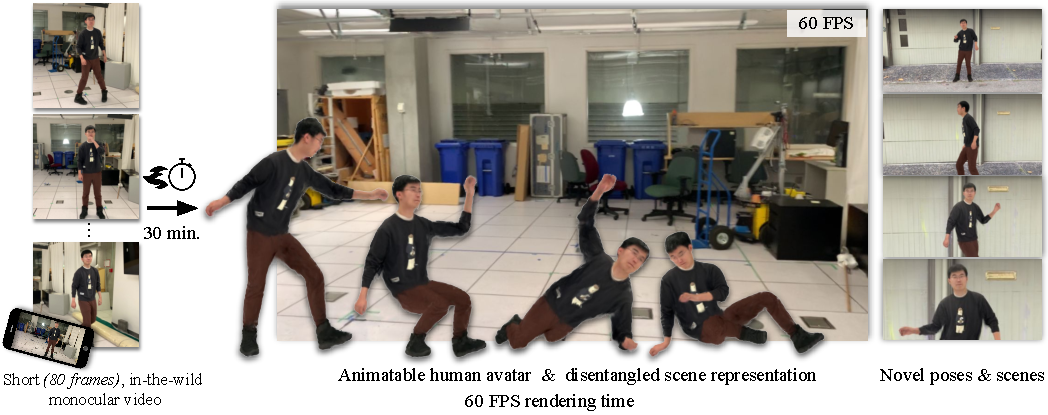
\includegraphics[width=\teaserwidth,clip]{figures/pdf_files/teaser.pdf}
		}
		\vspace{-1ex}
		\captionof{figure}{\textbf{Human Gaussian Splats (\acronym)} is a neural rendering framework that trains on 50-100 frames of a monocular video containing a human in a scene. HUGS enables novel view rendering with novel human poses at 60 FPS by learning a disentangled representation that can also render the human in other scenes. }
		% \vspace{-0.08in}
		\label{fig:teaser}
	\end{center}%
}]
\enlargethispage{2\baselineskip}
\begin{abstract}
Foundation model development attracts a rapidly expanding body of contributors, scientists, and applications.
To help shape \emph{responsible development practices}, we introduce the Foundation Model Development Cheatsheet: a growing collection of 250+ tools and resources spanning text, vision, and speech modalities.
We draw on a large body of prior work to survey resources (\emph{e.g.} software, documentation, frameworks, guides, and practical tools) that support informed data selection, processing, and understanding, precise and limitation-aware artifact documentation, efficient model training, advance awareness of the environmental impact from training, careful model evaluation of capabilities, risks, and claims, as well as responsible model release, licensing and deployment practices.
We hope this curated collection of resources helps guide more responsible development.
The process of curating this list, enabled us to review the AI development ecosystem, revealing what tools are critically missing, misused, or over-used in existing practices.
We find that (i) tools for data sourcing, model evaluation, and monitoring are critically under-serving ethical and real-world needs, (ii) evaluations for model safety, capabilities, and environmental impact all lack reproducibility and transparency, (iii) text and particularly English-centric analyses continue to dominate over multilingual and multi-modal analyses, and (iv) evaluation of systems, rather than just models, is needed so that capabilities and impact are assessed in context.  %\TODO{Finish one more point on systems vs models?}
% We hope this survey and review of resources will provide a practical guide to developers and a compass for meaningful future work in responsible AI.
\end{abstract}
% (\href{http://fmcheatsheet.org}{fmcheatsheet.org})
%%%%%%%%% BODY TEXT

\section{Introduction}
\label{sec:intro}

% The evolution of Large Language Models (LLMs)~\citep{gpt3,touvron2023llama,chatgpt} and vision foundation models~\citep{radford2021clip}
% has catalyzed advancements in constructing multi-modal intelligent agents capable of exploring the multi-modal realm, which are achieved by integrating LLMs and pre-trained vision encoders, followed by fine-tuning on image-text pairs~\citep{madureira-2021-flamingos,awadalla2023openflamingo} or specifically curated vision instruction-tuning datasets~\citep{liu2023llava,li2023m3it,Qwen-VL}.
% The evolution of Large Language Models (LLMs)~\citep{gpt3,touvron2023llama,chatgpt} and vision foundation models~\citep{radford2021clip} has catalyzed advancements in constructing intelligent agents capable of processing multi-modal information. 
Large vision-language models (LVLMs), which integrate large language models (LLMs)~\citep{gpt3,touvron2023llama} with pre-trained vision encoders through cross-modal alignment training~\citep{madureira-2021-flamingos,liu2023llava,li2023m3it}, 
have demonstrated remarkable perceptual and cognitive capabilities in processing concrete images from everyday scenes~\citep{gpt4v,fu2023mme,yang2023dawn,reka2024core}.
However, recent studies have shown that open-source LVLMs struggle to understand abstract figures, such as geometric shapes in multimodal mathematical reasoning~\citep{mathvista,zhang2024mathverse} and scientific plots~\citep{mmmu}. 
The inadequacy of training datasets in scientific domains that involve complex reasoning with abstract figures is the main underlying cause.
% This limitation stems from the scarcity of training datasets in scientific domains that incorporate complex reasoning involving abstract figures.
% , as most multi-modal instruction datasets focus on general images
% However, it remains unclear \lpk{if we know it's basically not satisfactory, then we can say it's not good rather than remains unclear} whether LVLMs can effectively reason over scientific figures and generate concise, human-like summary descriptions for paper figures. 
% This inquiry holds significance on two fronts: from a scientific perspective, it offers an ideal testbed for examining whether LVLMs can handle complex semantics involving reasoning processes that go beyond what is required by traditional vision question-answering~(QA) tasks. On a practical level, the implementation of a machine-assisted captioning tool could significantly enhance research efficiency, rendering scientific figures more accessible for individuals with visual impairments. \lpk{left here.}
% traditional vision-language tasks have 

To address this, we construct Multimodal ArXiv by utilizing the rich resources in preprints hosted on arXiv to improve the ability to understand scientific literature in LVLMs.
We first curate ArXivCap, a
diverse scientific figure-caption dataset.
In contrast to previous scientific figure datasets, which consist of synthesized figures~\citep{chen2020figcap}
or are restricted to simple captioning scenarios in the computer science domain~\citep{hsu-etal-2021-scicap-generating}, our dataset is composed of figures extracted from academic papers across a range of domains.
ArXivCap has 6.4M images and 3.9M captions from 572K papers. 
We also keep the subfigure structure, and titles of original papers, thereby supporting diverse evaluation tasks.
We further instruct GPT-4V to generate 100K multiple-choice question-answering~(QA) pairs for the figures in ArXivCap.
The resulting ArXivQA dataset could naturally serve as a pivotal resource for improving the scientific reasoning abilities of LVLMs.

We validate the effectiveness of our Multimodal ArXiv dataset from two dimensions: reasoning ability measured by QA accuracy and generation performance through novel vision-to-text tasks. 
Our experiments demonstrate that ArXivQA brings a significant 10.4\% absolute accuracy boost for Qwen-VL-Chat~\citep{Qwen-VL}, on the MathVista~\citep{mathvista}, a challenging benchmark for multimodal mathematical reasoning. 
Additionally, detailed analysis uncovers the relationship between paper domains and fine-grained task performance.
Moreover, using ArXivCap, we define four generation tasks of varying complexity to benchmark the ability of LVLMs to comprehend scientific plots:
(1) captioning a single academic figure, (2) generating overall summaries for multiple sub-figures, 
(3) in-context figure captioning given previous figure-caption pairs, and (4) generating paper titles from figure-caption pairs. 
We examine various LVLMs, including open-source models as well as proprietary models including GPT-4V~\citep{gpt4v} and Gemini 1.0 Pro Vision~\citep{team2023gemini}.
Evaluation results reveal that despite that current LVLMs still face challenges generating faithful captions for scientific figures, in-domain training on our dataset yields substantial performance improvements across all four tasks.
Manual error analysis underscores that LVLMs still suffer from misinterpretation of the visual context, recognition errors, and overly simplified captions, paving the way for future studies.
% \lpk{i hate say `something bad, while something good', i prefer say `despite something bad, something good' -- look at the brighter side :p}
% Evaluation results reveal that current LVLMs still face challenges generating faithful captions for scientific figures, while in-domain training on our dataset yields substantial performance improvements across all four tasks.





% In summary, we posit that our curated dataset and comprehensive experimental evaluation serve as a valuable resource for a thorough analysis and improvement of LVLMs' understanding of scientific figures, providing insights into the ongoing development of LVLMs.

% Specifically, .
% r by further pre-training with image-text pairs (Alayrac et al.;
% Awadalla et al., 2023) or by fine-tuning them with specialized vision instruction tuning datasets (Liu
% et al., 2023a; Zhu et al., 2023), leading to the emergence of powerful Large Multimodal Models



% OCR supplement training
\section{Related Work}

%Photorealistic rendering and animation of humans is an important area of research. 
Early works on photorealistic rendering and animation employed traditional computer graphics pipelines which involved large multi-camera setups such as lightstages ~\cite{debevec2012light} to capture the detailed texture and material of the human body. The animation of human bodies involved the rigging of an artist-created template of a human body mesh~\cite{alexander2013digitalira, alexander2010emily}. The introduction of statistical body shape models~\cite{anguelov2005scape, SMPL:2015, pavlakos2019smplx, STAR:ECCV:2020, SUPR} enabled representation of diverse human shape and animation of the human body by a single model. This reduced the manual effort in creating template meshes and rigging them.
%\jg{more quickly? More realistically? more easily? by non professionals?}. 
However, these shape models do not account for many details such as clothing, hair, accessories etc. Follow up works such as DRAPE~\cite{drape2012guan} or CAPE~\cite{ma2020cape} augment the shape models to add an additional layer of clothing or altogether choose a different representation such as occupancy~\cite{saito2019pifu, saito2020pifuhd, chen2021snarf, xiu2023econ, xiu2022icon} to represent the details of the geometry. This led to improved estimation of geometry, however the capturing appearance without large capture setups still remained a challenge.

In recent years, Neural Radiance Fields (NeRF)~\cite{mildenhall2020nerf} have enabled a joint representation of geometry and appearance for view-synthesis using multiview images without the need of a large capture setup. Although, a NeRF is designed for capturing static objects, recent work~\cite{peng2021neuralbody, weng2020vid2actor, liu2021neuralactor, weng2022humannerf, jiang2022neuman, Su21arxiv_A_NeRF, guo2023vid2avatar, Feng2022scarf,Mihajlovic:KeypointNeRF:ECCV2022} has extended the NeRF to enable capturing a dynamic moving humans
%by using a multi-camera setup in a capture lab. 
Weng et al.~\cite{weng2022humannerf} propose a method to model a NeRF representation of a human using a single monocular video enabling 360 degree view generation of a human. Furthermore, NeuMan~\cite{jiang2022neuman} introduces a joint NeRF representation of human and the scene capable of view synthesis and animation of the human in the scene. However, a major limitation of NeRF-based methods is that NeRFs are slow to train and render. Several methods have emerged to speed up training and rendering of NeRFs. These include using an explicit representation such as learning a function at grid points \cite{chen2022tensorf, reiser2021kilonerf}, using hash encoding \cite{muller2022instantngp} or altogether discarding the learnable component~\cite{fridovich2022plenoxels,liu2020neural}. 

Recent work on 3D Gaussian Splatting~\cite{kerbl3Dgaussians} uses a set of 3D Gaussians to represent a scene and renders it by splatting and rasterizing the Gaussians. This approach significantly improves the training and rendering times over traditional NeRFs. Recent work has addressed the extension of 3DGS scenes to controlled dynamic scenes~\cite{wu20234dgs} and multi-camera capture setup~\cite{luiten2023dynamicgs}. However, the 3D Gaussian Splatting framework is not trivial to extend to dynamic humans that allows for both novel-view and novel-pose synthesis of human and the scene.

Our methods builds on the 3D Gaussian Splatting framework~\cite{kerbl3Dgaussians} and utilize the \smpl body shape model~\cite{SMPL:2015} as a prior and learns a deformation model for animation control. 
We use a triplane and three MLPs to coordinate the Gaussians (\eg, their rotation, scale, color, and LBS weights). 
%
%We use a graph representation to bind the Gaussian points and use graph 
% \ar{No graph convs anymore. change this $\rightarrow$}
% convolutions~\cite{graph-conv, coma, cape} to regress the properties of the Gaussian points. 

%While neural fields have established themselves as state-of-the-art approach for representing static 3D scenes, the generalization to dynamic scenes, especially involving humans has been difficult.

%Traditional approaches for representing a human body mainly focused on geometry. Early works~\cite{SMPL:2015, CAPE} learn a mesh representation for humans and their clothing respectively. This enables 
%Following works such as PiFU~\cite{PiFU} use an implicit representation using an occupancy field~\cite{occupancy_nets} .

%GCN works coma, cape, meshcnn
%This problem is inherent to the structure-from-motion ambiguity where the camera motion and the object motion in the scene are entangled. To deal with this, recent approaches~\cite{neuralavatar_zju3d, neuralactor} use multi-camera setup in a capture lab to disentangle camera motion and human motion. 



\section{The CC-Layer}
\label{sec:implement}
\subsection{Constructing the CC-layer}
\label{sec:implement_construct}
Given a discrete feature map $\varbold{I}$ of shape $[N,C_{in},H,W]$, we are interested in a layer that produces $\varbold{I'}=CC\{\varbold{I}\}$ of shape $[N,C_{out},H',W']$ which is resized by a (non-integer) scale-factor $(s_h, s_w)$. Here $N$ is the batch-size, $C$ is the number of channels. $H,W$ are spatial dimensions. The desired spatial size $H',W'$ may be chosen at inference time.
Our CC-layer consists of 4 principled building blocks, marked by numbers in Fig.~\ref{fig:overview} (for simplicity, $I$ and $I'$ are drawn as 2D vectors in Fig.~\ref{fig:overview}, i.e.,  4D tensors with $N=1$ and $C=1$). These are described next:

\textbf{Block 1 -- Projected-grid:} 
The Projected grid \varbold{$\textbf{g}$} matches each output `pixel' $\textbf{n}$=$(i', j')$$\in$$I'$ to a sub-`pixel' location \varbold{$\textbf{g}_n$} in the continuous space of the \ben{input} $I$. This grid is captured by a tensor of shape $[2,H',W']$ where the the first dimension are the 2 projected sub-`pixel' coordinates (vertical and horizontal) of each output `pixel' $\textbf{n}$=$(i', j')$$\in$$I'$, and $H', W'$ are for all the output `pixels'.

%\michal{why don't we see the number of Fig.4 in the next paragraph?}

Let's start with a simple example. Fig.~\ref{fig:grid}.a depicts a standard 1D  downscaling by %an integer 
$2$. Note that even when the scale-factor $s$ is an integer (or an inverse integer: ${s=\ben{\nicefrac{1}{2}}}$ in this case), it is  \emph{wrong} to map an output `pixel' position $\textbf{n}$$\in$$I'$  to its input position in $I$ by simply multiplying (or dividing)  by the scale-factor $s$. It can be observed in Fig.~\ref{fig:grid}.a   that ${\varbold{\textbf{g}_n}\neq2\textbf{n}=\textbf{n}}/{s}$
%\ben{\nicefrac{\textbf{n}}{s}}}$.
To obtain the correct mapping, let's
define $d_{out}$  to be the distance of any output `pixel'  
%\textbf{n}$$\in$$I'$  
\michal{$\textbf{n}$}
from the leftmost boundary of $I'$.  $d_{out}$  is measured in units of output `pixels'. The matching coordinates \varbold{$\textbf{g}_n$}   in the \ben{input} $I$  is  defined to have a distance $d_{in}$ from the leftmost boundary of  $I$, and is measured in units of input `pixels'. The correct mapping rule across image scales~\cite{MATLAB:2010} is $d_{in}$=${d_{out}}/{s}$, 
since the total shape (from boundary-to-boundary) is resized, rather than discrete `pixel' centers. Since the first `pixel' \emph{center} (in any \ben{feature map/image}) is always half a `pixel' away from the leftmost boundary, hence:
%we can easily relate $d$ to $n$ and to $\varbold{\textbf{g}_n}$, by 
$d_{out}$=$n$+$\frac{1}{2}$  and  $d_{in}$=$\varbold{\textbf{g}_n}$+$\frac{1}{2}$.
%Plugging it in, we get the
This entails the
well known relation used in image resizing methods~\cite{MATLAB:2010}: 
%$ \varbold{\textbf{g}_n}$=$\frac{n}{s}$+$\frac{1}{2}$$\left(\frac{1}{s}-1\right)$
$ \varbold{\textbf{g}_n}$=$\frac{n}{s}$+$\frac{1}{2}$$(\frac{1}{s}$-$1).$

% \michal{the next paragraph is very tedious, can and SHOULD be shortened substantially.}
% However, we need to handle also non-integer output shapes. Such an example is illustrated in Fig.~\ref{fig:grid}.b. Since images or feature-maps  can only be represented  by integer-sized vectors/tensors, we will usually (but not always) determine the size of the output layer to be $out\_size =\lceil s \cdot in\_size \rceil$, However, the intrinsic (non-integer) output size $s \cdot in\_size$ must be kept, as this is the true size of the output, while the integer size contains an extra sub-`pixel' margin. Fig.~\ref{fig:grid}.b shows a projected grid for resizing a $4 \times 4$ input layer by 0.6 and 1.4,  respectively. The final output size ($3 \times 6$) is larger than the intrinsic size ($2.4 \times 5.6$), due to the ceiling $\lceil * \rceil$ operation. 
% % To prevent misalignments, we need to map each output `pixel' center to its correct input `pixel' center. For this we need to shift the output `pixels' by half of the margin $\textbf{n}=\textbf{n}' -(out\_size - in\_size \cdot s)/2$. Plugging this into the relation of $p$ to $p'$ we obtain:
% To prevent misalignments due to this added sub-`pixel' output margin, and guarantee that each output `pixel' center is mapped to its correct input location, we need to shift the output `pixels' by half of the added margin:  $\textbf{n}=\textbf{n}' -(out\_size - in\_size \cdot s)/2$. %Plugging this into the relation of $p$ to $p'$ we obtain:
% This yields the final accurate grid mapping:
However, we need to handle also non-integer output shapes. The intrinsic output size 
$s \cdot in\_size$ may not be an integer, yet images or feature-maps  can only be represented  by integer-sized vectors/tensors. We will usually (but not always) determine the size of the output $I'$ to be $out\_size =\lceil s \cdot in\_size \rceil$. Fig.~\ref{fig:grid}.b shows an example of a projected grid for resizing a $4 \times 4$ input \ben{feature map} by scales 0.6 and 1.4,  respectively. The final output size ($3 \times 6$) is larger than the intrinsic size ($2.4 \times 5.6$), due to the ceiling operation $\lceil$*$\rceil$.  Therefore, the final  grid mapping (which accurately covers all cases) is:
\begin{align}
    \varbold{g_n} = \frac{n}{s} + \frac{1}{2}\Big( in\_size - 1\Big) - \frac{1}{2s}\Big(out\_size-1\Big)    
    \label{eq:grid}
\end{align}
% Since every output `pixel', (i, j) is mapped to continuous 2D coordinates in the input feature-map, % Since the grid matches two location coordinates to each output `pixel', 
% it is a represented as a standard CNN tensor of order 4, with shape $[1,2,H',W']$, where 
% the batch size is 1. The second dimension is 2 for 2 spatial continuous coordinates in the input space and the last two are for the height and width of the output. 


% First we calculate a grid of sub-pixel coordinates, which matches output pixels locations in the input continuous space. Each output pixel is assigned to horizontal and vertical sub-pixel position in the input. This grid is a function purely of the scale-factors and the output shape. Thus, importantly, the grid can be determined at inference time dynamically.

% To accurately obtain the projected-grid, we need to acknowledge that discrete `pixels' have non-infinitesimal size, thus we distinguish between `pixel' ordinal numbers to continuous locations of their centers. Fig.~\ref{fig:grid}.a depicts a 1d standard downscaling by a factor of $\frac{1}{2}$. Note that it even when the downscalinfg/upscalingis by an integer scale-factor (2 in this case), it is wrong to map output `pixel' positions to input positions by directly multiplying by the scale-factor. We mark the discrete `pixel' coordinates by $p$ and the scale-factor by $s$. First we observe that $p' \neq sp$. In the figure it is clear that `pixel' 0 should not be mapped to output `pixel' 0, rather the boundary between `pixel' 0 to `pixel' 1. We define the distance from the left boundary as $d$ measured in units of full `pixel's. Since the first `pixel' center is half a `pixel' to the right with respect to the left boundary, $d=p+\frac{1}{2}$. To correctly resize, we need the total size of the input (4 in the example) to be mapped to the total size of the output, hence $d'=s \cdot d$. plugging in the relation between $p$ and $d$: $p'+\frac{1}{2} = s(p+\frac{1}{2})$ so that the mapping rule between input and output `pixels' is $p = \frac{p'}{s} + \frac{1}{2} \left( \frac{1}{s} - 1 \right)$.


% Next we need to handle non-integer output shapes. Since we can only represent images or feature-maps sizes as integers we will usually (but not always) determine the output size as $Ceil(s \cdot in\_size)$. However, the intrinsic size $s \cdot in\_size$ must be held. We point out that in some cases of resizing, it is crucial to specify both scale-factors and output shape. For example, in a sequence of resizing operations. Fig.~\ref{fig:grid}.b illustrates projected grid for resizing by 0.6 and 1.4 respectively. The final output size is thus bigger than the intrinsic size. Depending on the kernel support, the output can be influenced by `pixels' out of the image, thus padding policy is required. Any further operation conducted on the output feature-map should treat the intrinsic size and not the padded size. The most reasonable convention in such cases is to preserve the center of the feature-map so that it maps to the center of the output. For this we need to shift the output `pixels' by half of the margin $p'=p'' -(out\_size - in\_size \cdot s)/2$. To finally obtain the grid, we map integer output `pixel' locations to their projected sub-`pixel' location in the input, we get for each dimension with its own scale-factor, input shape and output shape: 
% \begin{align}
%     g_n = \frac{n}{s} + \frac{1}{2}\Big( in\_size - 1\Big) - \frac{1}{2s}\Big(out\_size-1\Big)    
%     \label{eq:grid}
% \end{align}
% Since every output `pixel', (i, j) is mapped to continuous 2D coordinates in the input feature-map, % Since the grid matches two location coordinates to each output `pixel', 
% it is a represented as a standard CNN tensor of order 4, with shape $[1,2,H',W']$, where 
% the batch size is 1. The second dimension is 2 for 2 spatial continuous coordinates in the input space and the last two are for the height and width of the output. 

\begin{figure}
%\vspace*{-0.5cm}
    \centering
    \hspace{-3cm}
    \begin{minipage}{.5\textwidth}
      \centering
      \hspace{1cm}
      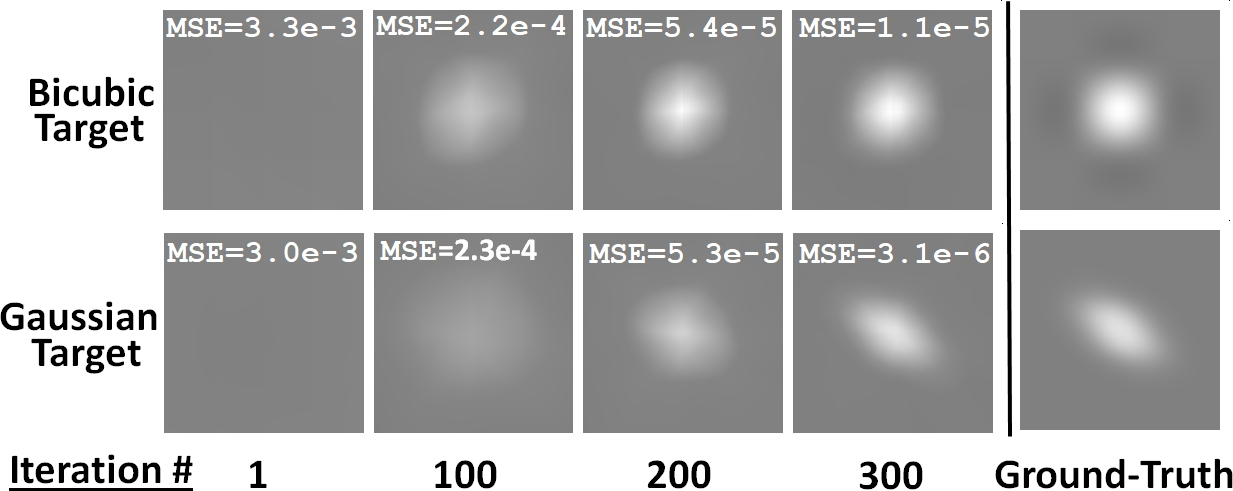
\includegraphics[width=1\textwidth]{figs/fig_visualize_Michal.jpg}
      \captionsetup{oneside, margin={-0.2cm,0cm}}
      \caption{\mbox{\it Visualizing the continuous learned kernels}}
      \label{fig:visualize}
    \end{minipage}
    \begin{minipage}{.4\textwidth}
        \vspace{-0cm}
        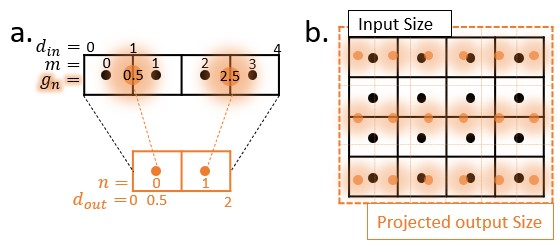
\includegraphics[width=1.5\textwidth]{figs/fig_grid.jpg}
        %\vspace*{0.5cm}
        \begin{minipage}{1.5\textwidth}
            \captionsetup{oneside, margin={1cm,0cm}}
            \caption{{\it The projected grid.}}
            \label{fig:grid}
         \end{minipage}%
    \end{minipage}%
    \vspace*{-0.5cm}
\end{figure}



\textbf{Block 2 -- Neighbors extraction:} For each grid point \varbold{$\textbf{g}_n$}, we now extract all its discrete nearest-neighbors $\varbold{\mathcal{N}[\textbf{n}]}$ \ben{from} $I$. These are all the input `pixels' centers within the support of the continuous kernel $\mathcal{K}_\theta$. This information is captured by a tensor of order 6 (blue tensor in Fig.~\ref{fig:overview}),  with shape $[N,1,C_{in},K,H',W']$ where K is the number of discrete neighbors in the kernel support. The second singleton dimension is for convenience in the next steps. We further need to extract the distances of each sub-`pixel' grid point \varbold{$\textbf{g}_n$} (of an output `pixel' {$\textbf{n}$}),  to all its discrete neighbors  ${\textbf{m}}\in I$. These distances $\varbold{\mathcal{D}[\textbf{n,m}]}$ are kept in a tensor $\varbold{\mathcal{D}}$ (shown in cyan in Fig.~\ref{fig:overview}), whose shape is $[K,2,H',W']$.

% Given a standard CNN input Tensor with dimensions Batch-size, Channels, Height and Width: $[N,C_{in},H,W]$.  We predefine support size (not necessarily an integer) for the continuous kernel $\mathcal{K}_\theata$. For each projected-grid point $\textbf{g'}$ we extract both values and distances to all input `pixels' within the kernel support. This stage produces a tensor consisting of all the neighbors values for each output `pixel'. This forces us to add a fifth dimension to the Neighbors tensor- the neighbors dimension. We actually extend this tensor to have 6 dimensions for convenience in the next stage, so the final shape is $[N,1,C_{in},K,H',W']$ where K is the number of neighbors in the kernel support. The Tensor of distances is shaped as a standard 2d CNN tensor, Its dimensions are: $[K,2,H',W']$. We use the batch dimension to distinguish between different neighbors. The second (channel) dimension is 2 to describe horizontal and vertical distances. Note that for simplicity, Fig.~\ref{fig:overview} depicts a case where $N=1, C_{in}=1$ and only the three last dimensions of the tensor are apparent.

% \textbf{Stage 3- Calculate weights:} The weights $\varbold{\mathcal{W}}$ are produced by the learnable model $\varbold{\mathcal{K}_\theta}$ applied to the distances tensor $\varbold{\mathcal{D}}$. 
\textbf{Block 3 -- Calculate weights:} The weights are produced by a learnable model $\varbold{\mathcal{K}_\theta}$, which is applied to the distances tensor:
%$\varbold{\mathcal{D}}$:
$\varbold{\mathcal{W} = \mathcal{K}_\theta \big\{ \mathcal{D}\big\}}$ (similarly to \cite{wang2018deep}).
A weight is assigned to connect between each output `pixel' and all its discrete input neighbors. Therefore, the weight tensor $\varbold{\mathcal{W}}$ will have a shape of $[1,C_{out},C_{in},K,H',W']$ 
(red tensor in Fig.~\ref{fig:overview}). 
%This tensor is marked in red in Fig.~\ref{fig:overview}. 
Its first singleton dimension is needed to match the size of the Neighbors tensor $\varbold{\mathcal{N}}$. As in standard conv, each output channel  $C_{out}$ is connected to all input channels $C_{in}$ through $\varbold{\mathcal{W}}$. We use a small neural network for $\varbold{\mathcal{K}_\theta}$ called the ``Internal-Net'' (marked in green in Fig.~\ref{fig:overview}). It is a simple CNN sequence of 1$\times$1 conv layers and ReLUs. This way every output `pixel' $\textbf{n}$ connects only to distances $\varbold{\mathcal{D}[\textbf{n}]}$ within its own set of discrete input neighbors. 

% The weights are produced by a learnable model which maps the distances calculated at stage 2 to corresponding weights for all the neighbors. This enforces consistency alongside expressivity. While each output `pixel' is calculated using a distinct local discrete kernel, all these local kernels are governed by the same underlying mapping function. We can choose to use a predefined fixed mapping, but we will usually use a learnable neural network, referred to as the internal-net. The input will be the distances tensor from preious stage. since we force the same mapping function to each output `pixel' we use several 1$\times$1 convolution layers and ReLUs in the internal-net. Consistency of the mapping to different neighbors is also enforced, since different neighbors are different instances in a batch. However, any model can be plugged to calculate the weights. Like in standard discrete convolutions, we have a set of continuous kernels, each maps all the input channels to an output channel. The weighted sum is actually taken not only over the neighbor values, but also over the input channels. Similarly to the neighbors tensor, the final weights tensor is of order 6: $[1,C_{out},C_{in},K,H',W']$ where the first dimension is the batch dimension which is always 1, to match the neighbors tensor.

\textbf{Block 4 -- Apply weights:} The final stage executes Eq.~\ref{eq:underlying} for the entire output tensor,
by multiplying the Weights tensor (red) with the Neighbors tensor (blue) and summing over all neighbors and input channels:
%. We simply multiply the Weights tensor (red) with the Neighbors tensor (blue) and sum over all the neighbors and input channels:
% For a given input feature-map $I$ of size $[N,C_{in},H,W]$, scale-factors $s_h, s_w$ and wanted shape $H',W'$ given at inference we finally get: 
\vspace*{-0.4cm}
\begin{align}
\varbold{I'}=
CC\{\varbold{I}\}= \sum_{c_{in}, k} \varbold{\mathcal{N}} \otimes \varbold{\mathcal{W}}
\end{align} 
with the following tensor shapes: 

$ \varbold{I'}:[N,C_{out},H',W'], \quad \varbold{\mathcal{N}}: [N,1,C_{in},K,H',W'], \quad \varbold{\mathcal{W}}:[1,C_{out},C_{in},K,H',W'] $

\subsection{Training and Generalization}
\label{sec:train}
CC is end-to-end trainable. The only trainable parameters of CC are $\varbold{\theta}$,  the parameters of $\varbold{\mathcal{K}_\theta}$. The gradient is propagated from the CC output through the weights tensor $\varbold{\mathcal{W}}$ to them. Gradients need to also be propagated to previous layers through the CC input. This is done easily through the neighbors extraction since it is just slicing (each neighbour neuron is actually a copy of an input neuron).

The output shape is determined by the shape of the grid $\varbold{{g}}$. Since $\varbold{\mathcal{K}_\theta}$ is a fully convolutional network, it can be applied to any spatial input size both at training and inference. This means that regardless of what sizes and scales we train on, a single CC, with a single set of parameters $\varbold{\theta}$ is applicable to any size and scale determined at real-time.

The input to  $\varbold{\mathcal{K}_\theta}$ is 
$\varbold{\mathcal{D}}$, which through the grid  $\varbold{{g}}$ depends only on the desired output scale \&
shape. Naturally, to generalize to many scales, we can sample various scales during training. However, being fully 1$\times$1 convolutional, $\varbold{\mathcal{K}_\theta}$ actually maps every 2D distance vector
%distance (two coordinates -- vertical and horizontal)
$\varbold{\mathcal{D}[\textbf{n,m}]}$ to a single value (weight) $\varbold{\mathcal{W}[\textbf{n,m}]}$. This means that $\varbold{\mathcal{D}}$ actually contains a huge batch of
inputs. This produces an interesting advantage: in almost all cases CC generalizes from one scale to any other scale. This happens as long as the diversity of distances in a single grid is reasonable. Eq.~\ref{eq:grid} suggests that if the scale is a rational number with a small numerator, 
then there exists only a small set of grid coordinates, and consequently a small set of unique distances $\varbold{\mathcal{D}[\textbf{n,m}]}$. For example, for $s=\nicefrac{1}{2}$ and a kernel with support of 2$\times$2, we get:
%\rightarrow 
$\varbold{\mathcal{D}[\textbf{n}]} = \Big\{(-\nicefrac{1}{2},-\nicefrac{1}{2}), 
(-\nicefrac{1}{2},\nicefrac{1}{2}), 
(\nicefrac{1}{2},-\nicefrac{1}{2}), 
(\nicefrac{1}{2},\nicefrac{1}{2})
\Big\} \ \ \varbold{\forall \textbf{n}}$, which will not generalize to other scales/distances. In other words, generalization occurs over the distribution of distances $\varbold{\mathcal{D}}$  between the grid points and `pixel' centers. If this distribution collapses to a small set of possibilities, then such generalization is damaged. However, training with a \emph{randomly} selected float scale-factor will give a huge diversity of sub-`pixel' distances in $\varbold{\mathcal{D}}$, hence will be able to generalize with very high probability to any other scale factor.
%\michal{Is this still true for large gaps between the train-scale  and the test-scale? After all, this will lead to a large difference in support size of K}. \assaf{supprt size of K is independent of the scale} 
Empirical evaluation of this property is described in the experiments section and in Fig.~\ref{fig:generalize}.
%\michal{Reference to Fig. 7 broken}
% \textbf{Cross-scale generalization:} Since the learning model $\mathcal{K}_\theta$ is unaware of the scale, it can be trained to one scale and generalize to another, under reasonable conditions. the scale trained on, cannot be a special case that collapses back to convolution, or a rational number with a denominator that is too small. In other words, generalization occurs over the distribution of distances between the grid and `pixel' centers. If this distribution collapses to a small set of possibilities then such generalization is damaged. A randomly selected float scale-factor will be able to generalize with probability ~1. 


% \textcolor{red}{
% \subsection{Training the CC-layer for dynamic scale generalization}
% \begin{itemize}[leftmargin=0.7cm]
% \item Please explain how to train the CC-layer so that it can generalize at test-time to any desired scale and shape.
% \item Please stress that although we use many scale/shape augmentations of the output layer, this is still a single trained network (as opposed to training multiple different networks, each for a different fixed output scale/shape). This is obvious to us, but may be a natural misconception of the reviewers, so it is worth stressing. Better safe than sorry...
% \end{itemize}
% }
\section{Constructing a scaling testbed}
\label{sec:experiments}

\begin{figure}[tp]
    \centering
    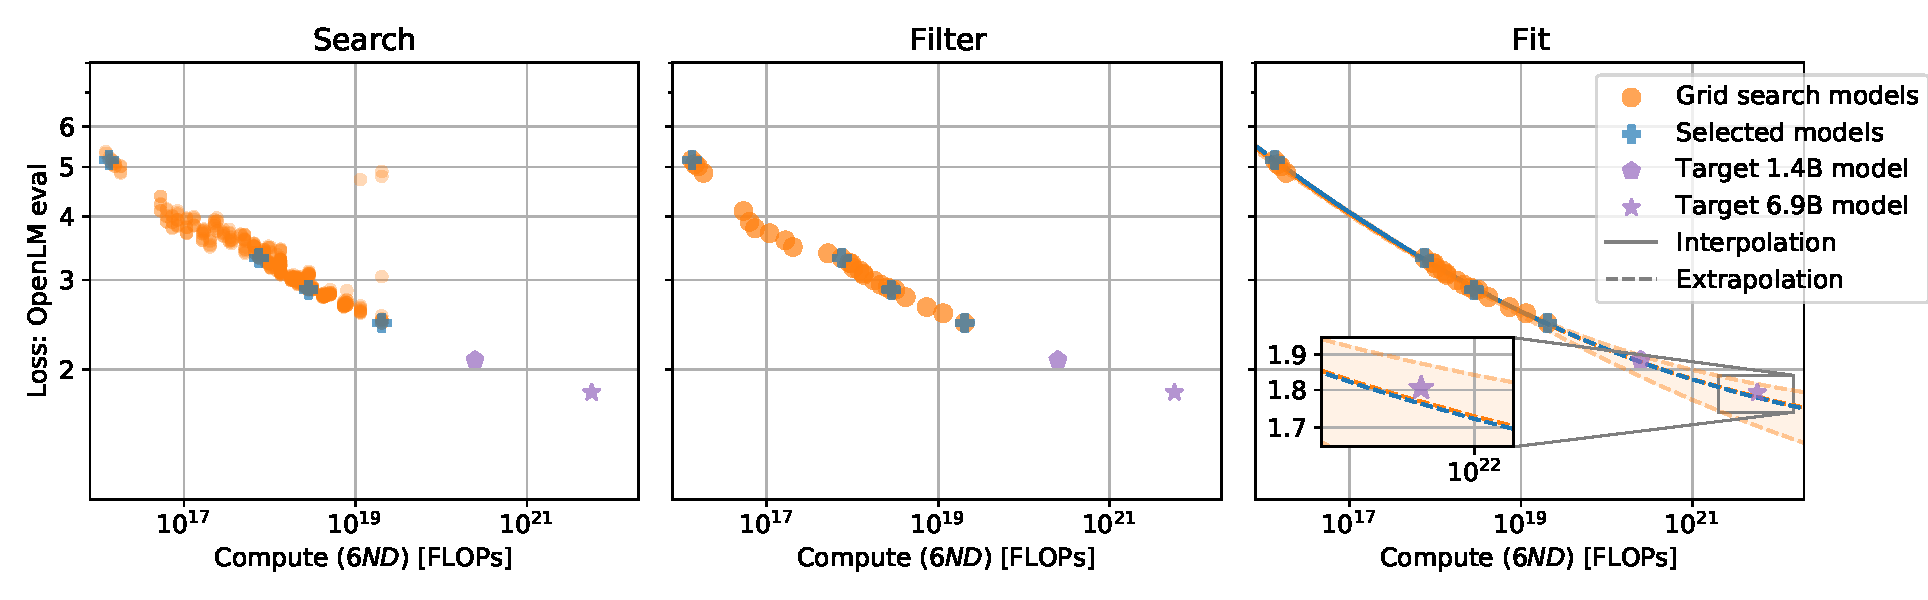
\includegraphics[width=\linewidth]{figs/grid_full.pdf}
    \caption{\textbf{Search, filter, fit:
    A recipe for selecting configurations for scaling.}
    \emph{(left)} To generate the final configurations presented in Table~\ref{tab:hparams}, we run a 435 model grid search over model width, hidden dimension, number of attention heads, batch size, and warmup steps.
    All models are trained near compute-optimally.
    \emph{(center)} We plot the efficient frontier of models, which appear to follow a trend, excluding models from $5.2 \times 10^{16}$ to $5.2 \times 10^{17}$, which fall below the trend.
    \emph{(right)} We fit a power law with irreducible error to the remaining configurations, picking four configurations that closely track the full model suite (``Selected models'').
    These models extrapolate the performance of 1.4B, 6.9B target models.
    Shaded regions represent bootstrap 95\% confidence intervals.
    }
    \label{fig:grid}
\end{figure}

In this section, we discuss our experimental setup to test the predictions suggested by Equations~\eqref{eq:lossCM} and~\eqref{eq:errL}.
We first present our general language modeling setup (Section~\ref{sec:training}).
Next, we discuss our strategy for determining model configurations for our scaling investigation (Section~\ref{sec:searching}) and fitting scaling laws (Section~\ref{sec:fitting}).
We then present metrics to validate how well scaling laws predict loss and downstream performance (Section~\ref{sec:evaluation}).

\subsection{Training setup}
\label{sec:training}

We train transformers~\cite{transformer} for next token prediction, based on architectures like GPT-2~\cite{Radford2019LanguageMA} and LLaMA~\cite{llama}.
We employ GPT-NeoX~\cite{neox} as a standardized tokenizer for all data.
See Appendix~\ref{appx:additional_training_main} for architecture, optimization, and hyperparameter details.

\subsection{Model configurations}
\label{sec:searching}

To get final configurations for the 0.011B to 0.411B parameter models plotted in Figures~\ref{fig:emperical} and~\ref{fig:downstream_corr}, we first conduct a wide grid search over a total of 435 models, trained from scratch, from 0.01B to 0.5B parameters (Figure~\ref{fig:grid}~\emph{(left)}).
We train on the original OpenLM data mix~\cite{open_lm}, which largely consists of RedPajama~\cite{rpj} and The Pile~\cite{pile}.
While we eventually plan to over-train models, at this step we search for \emph{base configurations} near compute-optimality.
We train on 20 tokens per parameter ($M=20$), which, in early experiments, gives models near the compute-optimal frontier.
This is similar to findings in \citet{chinchilla}'s Table 3, which suggests that $M=20$ is near-optimal for the Chinchilla experimental setup.

To find maximally performant small-scale models on validation data, we tune model width, number of layers, number of attention heads, warmup steps, and batch size.
Our validation set, OpenLM eval, contains tokens from recent arXiv papers, the OpenLM codebase itself, and news articles.
We find in early experiments that qk-LayerNorm makes models less sensitive to learning rate, which is a phenomenon \citet{wortsman2023small} report in their Figure 1.
Hence, we fix the learning rate (3$e$-3) for our sweeps.
We also perform smaller grid searches over 1.4B and 6.9B parameter model configurations at $M=20$, retaining the best configurations.

At this point, we have many models, several of which give poor performance; following prior work~\cite{kaplan2020scaling,chinchilla}, we want to keep only models that give best performance.
Hence, in Figure~\ref{fig:grid}~\emph{(center)}, we filter out models that do not lie on the Pareto frontier.
While there appears to be a general trend, configurations between $5.2 \times 10^{16}$ and $5.2 \times 10^{17}$ FLOPs lie below the frontier established by other models.
We hypothesize these models over-perform as they are trained for more optimization steps than their neighbors based on our power-of-two batch sizes.
We provide support for this hypothesis in Appendix~\ref{appx:more_results}, but opt to remove these models from our investigation.

To ensure tractable compute requirements for our scaling experiments, we require a subset of models that follows the trend of the entire Pareto frontier.
In Figure~\ref{fig:grid}~\emph{(right)}, we fit trends to the Pareto models and to a subset of four models.
We notice that the trends closely predict both the performance of the 1.4B and 6.9B models, suggesting that our small-scale configurations reliably extrapolate in the compute-optimal setting.

Moving forward, we do not tune hyperparameters for other token multipliers (i.e., $M \neq 20$), on other training or evaluation distributions, or on validation sets for downstream tasks.
For more details including specific hyperparameters, see Appendix~\ref{appx:additional_training}.

To create our scaling testbed, we start with the four small-scale, base configurations from our grid search: $N\in \{0.011\text{B}, 0.079\text{B}, 0.154\text{B}, 0.411\text{B}\}$.
To ensure our conclusions are not particular to a single training distribution, we train models on each of C4~\cite{c4,c4_ai2}, RedPajama~\cite{rpj}, and RefinedWeb~\cite{refinedweb}, which have 138B, 1.15T, and 600B tokens, respectively, for different token multipliers $M \in \{5, 10, 20, 40, 80, 160, 320, 640\}$.
We omit runs that require more tokens than are present in a dataset (i.e., $N=0.411\text{B}, M=640$ for C4).
We additionally train $N=1.4$B models at $M=20$ and at the largest token multiplier possible without repeating tokens (i.e., 80 for C4, 640 for RedPajama, and 320 for RefinedWeb).
We train $N=6.9\text{B}, M=20$ models on each dataset given the relevance of 7B parameter models~\citep{llama,jiang2023mistral}.
In total this results in a testbed of 104 models.

\subsection{Fitting scaling laws}
\label{sec:fitting}

\begin{table}[tp]
    \centering
    \small
    \caption{\textbf{Default number of parameters $N$ and token multiplier $M$ to fit our scaling laws.}
    We invest $\sim$100 A100 hours to fit Equation~\eqref{eq:lossCM} and $\sim$1,000 A100 hours to fit Equation~\eqref{eq:errL}.} 
    % \vspace*{3mm}
    \begin{tabular}{lccc}
        \toprule
        $N$ & $M$ & Used to fit Equation~\eqref{eq:lossCM} & Used to fit Equation~\eqref{eq:errL} \\\midrule
        0.011B & 20 & \ding{51} & \ding{51}\\
        0.079B & 20 & \ding{51} & \ding{51}\\
        0.154B & 20 & \ding{51} & \ding{51}\\
        0.411B & 20 & \ding{51} & \ding{51}\\
        0.011B & 320 & \ding{51} & \ding{51}\\
        1.4B & 20 & \ding{55} & \ding{51}\\\midrule
        \multicolumn{2}{c}{Total compute $C$ [FLOPs]} & 2.4$e$19 & 2.7$e$20 \\\bottomrule
    \end{tabular}
    
    \label{tab:fit_hparams}
    % \vspace*{-3mm}
\end{table}
We fit Equation~\eqref{eq:lossCM} to approximate $E, a, b, \eta$ using curve-fitting in SciPy~\cite{scipy} (i.e., Levenberg-Marquardt to minimize non-linear least squares).
We repeat this process to fit Equation~\eqref{eq:errL} to approximate $\epsilon, k, \gamma$.
We invest $\sim$100 A100 hours to train the models required to fit a scaling law for loss and $\sim$1,000 A100 hours for a corresponding law for downstream error.
Unless otherwise specified, we fit to the $N, M$ pairs in Table~\ref{tab:fit_hparams}, which are a subset of our full testbed.
Our configurations allow us to test for extrapolation to the $N=1.4\text{B}, M=640$ (900B token) and the $N=6.9\text{B}, M=20$ (138B token) regimes.

\subsection{Evaluation setup}
\label{sec:evaluation}

\paragraph{Evaluation datasets.}
Unless otherwise stated, our default validation loss dataset is C4 eval.
For downstream tasks, we adopt a subset from 46 tasks from LLM-foundry~\cite{mosaicml}, which includes standard tasks with both zero-shot and few-shot evaluations.
Specifically, we consider a 17-task subset where, for each evaluation, at least one 0.154B scale model---trained with as many as 99B tokens---gets 10 percentage points above chance accuracy:
ARC-Easy~\cite{arc},
BIG-bench: CS algorithms~\cite{srivastava2023beyond},
BIG-bench: Dyck languages~\cite{srivastava2023beyond},
BIG-bench: Novel Concepts~\cite{srivastava2023beyond},
BIG-bench: Operators~\cite{srivastava2023beyond},
BIG-bench: QA WikiData~\cite{srivastava2023beyond},
BoolQ~\cite{boolq},
Commonsense QA~\cite{talmor-etal-2019-commonsenseqa},
COPA~\cite{copa},
CoQA~\cite{reddy-etal-2019-coqa},
HellaSwag (zero-shot)~\cite{hellaswag},
HellaSwag (10-shot)~\cite{hellaswag},
LAMBADA~\cite{lambada},
PIQA~\cite{piqa},
PubMed QA Labeled~\cite{pubmed},
SQuAD~\cite{squad},
and
WinoGrand~\cite{winograd}.
For more details on evaluation datasets see Appendix~\ref{appx:eval_data}.
We focus on this subset to ensure we are measuring signal, not noise.
Including downstream tasks like MMLU~\cite{mmlu}, where performance is close to random chance, however, does not invalidate our results as we show in our evaluation set ablations (Appendix~\ref{appx:more_results}).

\paragraph{Metrics.}
We consider three main metrics:
\emph{Validation loss}, which is the cross entropy between a model's output and the one-hot ground truth token, averaged over all tokens in a sequence and over all sequences in a dataset.
\emph{Average top-1 error}, which is a uniform average over the 17 downstream evaluations, as mentioned in the above paragraph.
To measure how good a prediction $\zeta(C, M)$ is, we measure \emph{Relative prediction error}: $|\zeta(C, M) - \zeta_{GT}| / \zeta_{GT}$, where $\zeta$ is the predicted loss $L$ or the average top-1 error $\textsf{Err}$. $\zeta_{GT}$ is the ground truth measurement to predict.

\section{Results: Reliable extrapolation}
\label{sec:results}

In this Section, we quantify the extent to which the scaling laws developed in Section~\ref{sec:method} extrapolate larger model performance using the scaling testbed from Section~\ref{sec:experiments}.
By default, we fit Equations~\eqref{eq:lossCM} and~\eqref{eq:errL} to the configurations in Table~\ref{tab:fit_hparams}, use C4 eval for loss, and the 17-task split from Section~\ref{sec:evaluation} for average top-1 error.
% \vspace*{-2mm}
\begin{figure*}[tp]
    \centering
    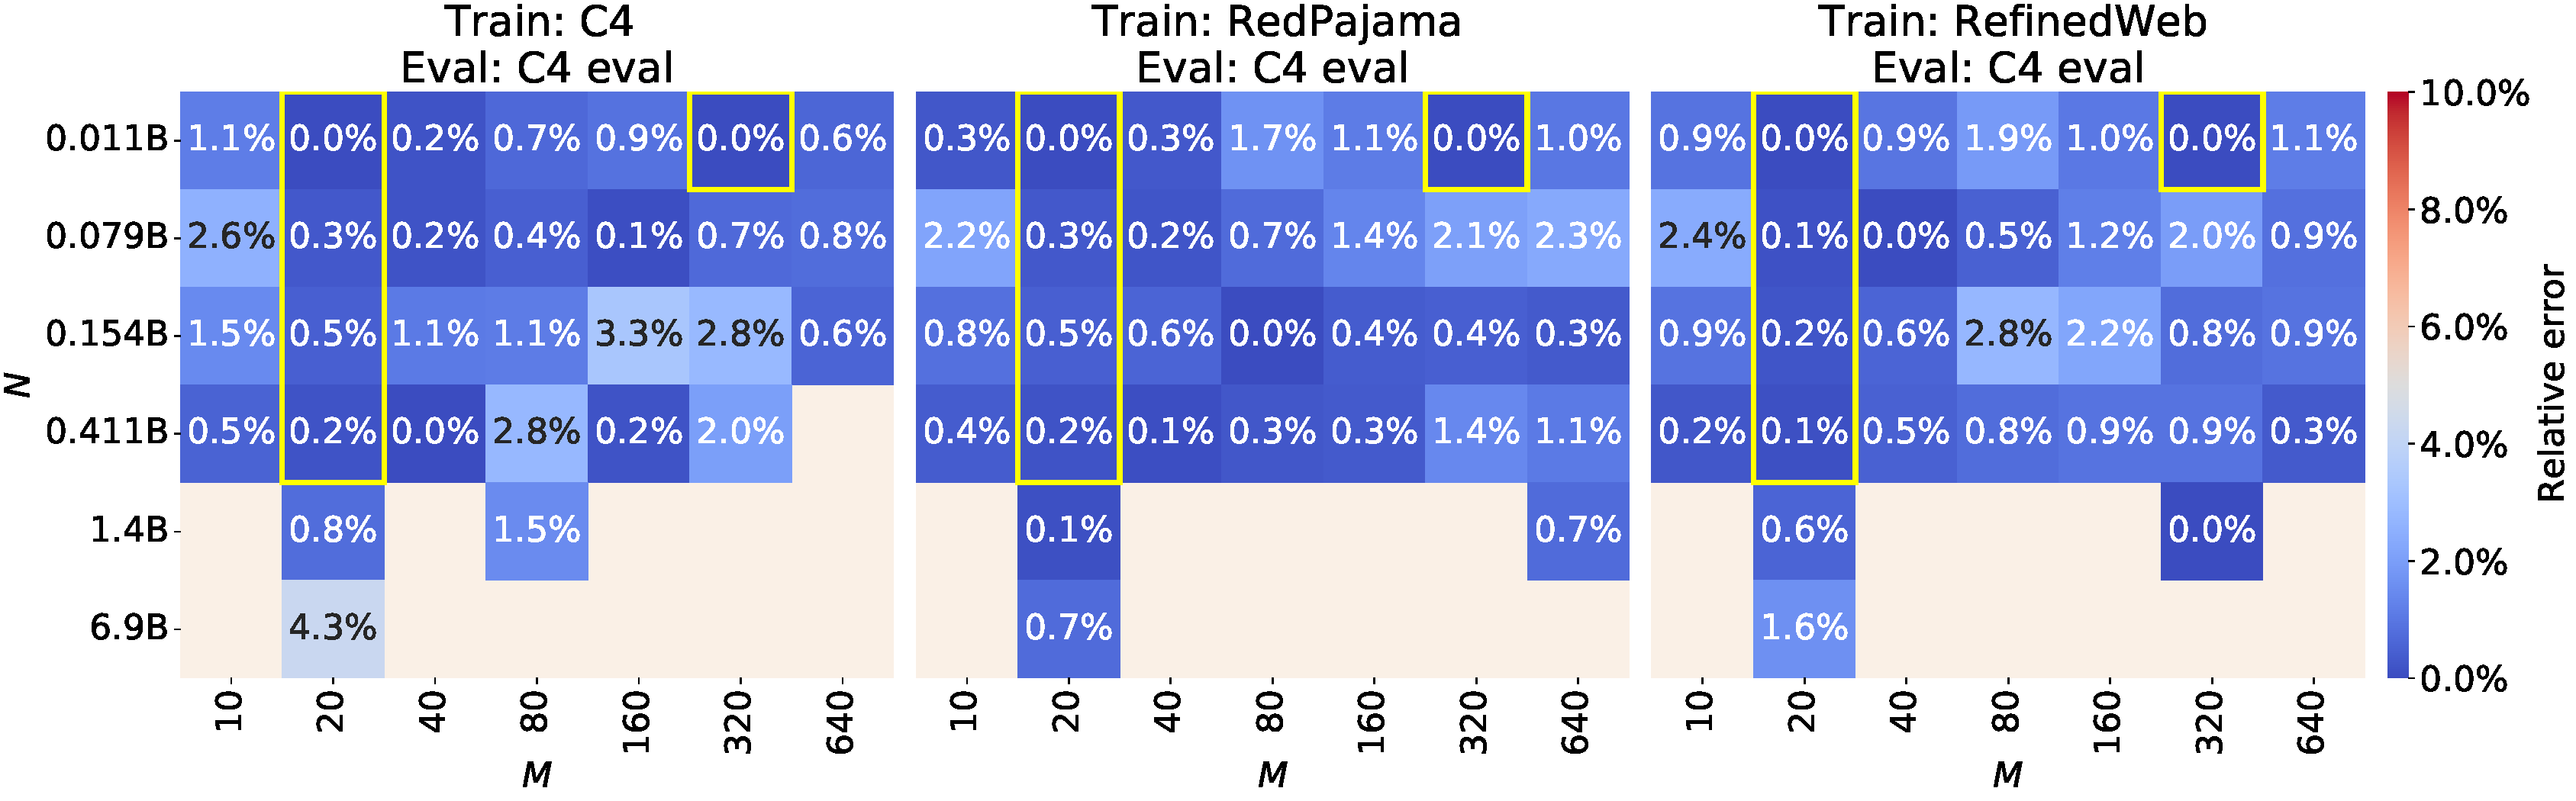
\includegraphics[width=\linewidth]{figs/error.pdf}
    \caption{\textbf{Relative error on C4 eval for different training distributions.} Boxes highlighted in yellow correspond to pairs---number of parameters $N$, token multiplier $M$---used to fit Equation~\eqref{eq:lossCM}. Larger values of $M$ correspond to more over-training. The prediction error is low in both interpolation and extrapolation ranges. Below $N=1.4$B, empty squares correspond to runs that were not possible due to the limited dataset size for single epoch training. At $N=1.4$B we run at $M=20$ and at the largest possible multiplier. At $N=6.9$B, we run at $M=20$.}
    \label{fig:error}
    % \vspace*{-2mm}
\end{figure*}

\paragraph{Over-trained performance is predictable.}
We highlight our main over-training results in Figure~\ref{fig:fig1}~\emph{(left)}.
Namely, we are able to extrapolate both in the number of parameters $N$ and the token multiplier $M$ to closely predict the C4 eval performance of a 1.4B parameter model trained on 900B RedPajama tokens ($N=1.4\text{B}, M=640$).
Our prediction, which takes 300$\times$ less compute to construct than the final 1.4B run, is accurate to within 0.7\% relative error.
Additionally, for the $N=6.9\text{B}, M=20$ run, near compute-optimal, the relative error is also 0.7\%.

These results support several key takeaways.
(i) Scaling can be predictable even when one increases both the model size and the amount of over-training compared to the training runs used to fit a scaling law.
(ii) The form presented in Equation~\eqref{eq:lossCM} is useful in practice for predicting over-trained scaling behavior.
(iii) Fitting to Equation~\eqref{eq:lossCM} gives good prediction accuracy near compute-optimal.
More specifically, predictions are accurate both for the 1.4B over-trained model and the 6.7B compute-optimal model using a single scaling fit.

While Figure~\ref{fig:fig1} explores a specific case of making predictions in the over-trained regime, we aim to understand the error profile of our predictions across training datasets, token multipliers, and number of parameters.
Hence, Figure~\ref{fig:error} shows the relative error between ground truth loss and predicted loss on C4 eval for models in our testbed.
We notice uniformly low prediction error suggesting that predictions are accurate in many settings.

% \vspace*{-2mm}
\paragraph{Average top-1 error is predictable.}
Figure~\ref{fig:fig1}~\emph{(right)} presents our main result in estimating scaling laws for downstream error.
Concretely, we use the models indicated in Table~\ref{tab:fit_hparams} to fit Equations~\eqref{eq:lossCM} and~\eqref{eq:errL}, chaining the scaling fits to predict the average top-1 error as a function of training compute $C$ and the token multiplier $M$.
Our fits allow us to predict, using $20\times$ less compute, the downstream performance of a 6.9B model trained on 138B RedPajama tokens to within $0.05\%$ relative error and a 1.4B model trained on RedPajama 900B tokens to within $3.6\%$ relative error.

Table~\ref{tab:downstream} additionally shows the relative error of our downstream performance predictions for models trained on C4, RedPajama, and RefinedWeb, indicating that our scaling law functional forms are applicable on many training datasets.
We note that while average accuracy is predictable, \textit{individual} downstream task predictions are significantly more noisy.
We report relative error for more model predictions in Figures~\ref{fig:error_downstream_all} and \ref{fig:error_downstream_subset}.
We also find that if we remove the 1.4B model for the Equation~\eqref{eq:errL} fit, relative error jumps, for instance, from 0.05\% to 10.64\% on the 17-task split for the 6.9B, 138B token RedPajama prediction.
This highlights the importance of investing more compute when constructing scaling laws for downstream task prediction compared to loss prediction.

\begin{table}[tp]
    \centering
    \caption{
    \textbf{Downstream relative prediction error at 6.9B parameters and 138B tokens.}
    While predicting accuracy on individual zero-shot downstream evaluations can be challenging (``Individual''), predicting \textit{averages} across downstream datasets is accurate (``Avg.'').
    }    
    \resizebox{\linewidth}{!}{
    \begin{tabular}{lcccc@{\hskip 8ex}c}
        \toprule
        & \multicolumn{4}{c}{Individual top-1 error} & {Avg. top-1 error} \\
        \cmidrule(lr){2-5} \cmidrule(lr){6-6}
         Train set & ARC-E~\cite{arc} & LAMBADA~\cite{lambada} & OpenBook QA~\cite{OpenBookQA2018} & HellaSwag~\cite{hellaswag} & 17-task split \\\midrule
         C4~\cite{c4,c4_ai2} & 28.96\% & 15.01\% & 16.80\% & 79.58\% & 0.14\% \\
         RedPajama~\cite{rpj} & 5.21\% & 14.39\% & 8.44\% & 25.73\% & 0.05\% \\
         RefinedWeb~\cite{refinedweb} & 26.06\% & 16.55\% & 1.92\% & 81.96\% & 2.94\% \\ 
        \bottomrule
    \end{tabular}
    }
    % \vspace*{2mm}
    \label{tab:downstream}
    % \vspace*{-6mm}
\end{table}

% \vspace*{-3mm}
\paragraph{Under-training, out-of-distribution scaling, compute-reliability trade-offs.}
In addition to our main results presented above, we include additional results in Appendix~\ref{appx:more_results}, which we summarize here.
First, we notice that when token multipliers become too small (i.e., $M=5$) scaling becomes unreliable and lies off the trend.
Additionally, multipliers other than 20, such as 10, 40, and 80, garner points that are roughly on the compute optimal frontier (Figure~\ref{fig:emperical_small}).
This observation suggests that the compute-optimal multiplier may lie in a range rather than take a single value.
To probe the limits of reliable scaling, we attempt to break our scaling laws in out-of-distribution settings.
We find that models trained on C4---English filtered---and evaluated on next token prediction on code domains have a high relative error in many cases. Perhaps surprisingly, evaluating the same models on German next token prediction gives reliable loss scaling (Figure~\ref{fig:error_ood}).
We additionally examine the compute necessary to create accurate scaling laws, finding
that scaling laws can be constructed more cheaply for loss prediction than for downstream error prediction (Figures~\ref{fig:error_vs_1b} and~\ref{fig:error_vs_7b}).


% \input{sections/05_results}

\section{Related Work}

Srivastava et al. \cite{srivastava2022beyond} observed that while accuracy at a particular task can empirically appear sharp and unpredictable, cross entropy does not; the authors then hypothesized that emergent abilities may be partially attributed to the metric.
%writing: ``[Emergent abilities frequently appear] on tasks that have brittle or narrow metrics for success, emphasizing the importance of engineering graded metrics that can capture subthreshold improvements. Our results suggest that breakthrough performance can also occur on tasks that involve multistep reasoning. One possible explanation for the breakthrough phenomenon on multistep tasks is that the probability of success on the task scales like the product of the success probabilities on each step.”
Our paper converts their discussion into precise predictions, then quantitatively tests the predictions to reveal that: metric choice is likely wholly responsible for emergent abilities; well-known and widely-used metrics (including ones already used by \cite{srivastava2022beyond}) capture graded improvements; emergent abilities do not appear only for tasks involving multiple steps, and indeed appear most commonly on the discontinuous Multiple Choice Grade; metric choice can be used to induce emergent abilities in a novel domain (vision) in diverse architectures and tasks.

Caballero et al. \cite{caballero2022broken} explain emergence by assuming a piece-wise power law functional form; under this view, emergent abilities are real, caused by a change in the governing power law. In contrast, our work suggests that emergent abilities are induced by the researcher, even under a single power law. Michaud et al. \cite{michaud2023quantization} posit that emergent abilities may be real under strong data assumptions.

\section{Discussion}

Our paper presents an alternative explanation for claimed emergent abilities of large language models. For a fixed task and a fixed model family, the researcher can choose a metric to create an emergent ability or choose a metric to ablate an emergent ability. Ergo, \textit{emergent abilities may be creations of the researcher's choices, not a fundamental property of the model family on the specific task.} We emphasize that nothing in this paper should be interpreted as claiming that large language models \textit{cannot} display emergent abilities; rather, our message is that previously claimed emergent abilities in \cite{brown2020language, ganguli2022predictability,srivastava2022beyond,wei2022emergent} might likely be a mirage induced by researcher analyses.

Our paper has several implications. Firstly, a task and a metric are distinct and meaningful choices when constructing a benchmark. Secondly, when choosing metric(s), one should consider the metric's effect on the per-token error rate and adapt their measuring process accordingly, e.g., if one chooses accuracy, one should make sure to have sufficient data to accurately measure accuracy to avoid the risk of drawing invalid scientific conclusions.
%Thirdly, what metrics \textit{should} one choose? If the goal is to measure how useful a model's outputs are to humans, then harsh metrics like Accuracy or Multiple Choice Grade may diverge from human preferences.
%For instance, suppose that Model A places 5\% probability mass on a Yes/No question's correct answer, and Model B places 40\% probability mass on the correct answer; under Multiple Choice Grade, these two models score equivalently: 0. To offer one real-world anecdote, while learning how to use BIG-Bench, the authors accidentally discovered within BIG-Bench a question ``Q: What is 4 plus 5?" and a model's answer ``The sum of 4 and 5 is 9" that was scored as 0 because regex is used to extract the first occurring integer.
%Consequently, determining to what extent common NLP metrics correlate with human preferences should be a priority to avoid overfitting to NLP metrics.
Thirdly, when making claims about capabilities of large models, including proper controls is critical. In this particular setting, emergent abilities claims are possibly infected by a failure to control for multiple comparisons. In BIG-Bench alone, there are $\geq$ 220 tasks, $\sim 40$ metrics per task, $\sim10$ model families, for a total of $\sim 10^6$ task-metric-model family triplets, meaning probability that \textit{no} task-metric-model family triplet exhibits an emergent ability by random chance  might be small.
Fourthly, scientific progress can be hampered when models and their outputs are not made public for independent scientific investigation.

% TODO: Decide whether to keep this or move to appendix. Our findings reveal that metrics exhibiting apparent emergence disproportionately penalize smaller-scale models. 
% Monitoring alternative metrics unveil consistent, predictable alterations as the model scales. 
% Consequently, small-scale experimentation remains valuable, provided appropriate metrics are employed to avoid undue penalization. 
% Specifically, GPT-4 development incorporated small-scaling experimentation alongside scaling laws [1].


% Commented out for NeurIPS

% \section{Contributions}

% RS conceived of the research direction, collected data, ran experiments and analyzed results. SK supervised and guided the project. BM also provided guidance.

% \section{Acknowledgements}

% We thank our colleagues Max Lamparth, Mikail Khona, Kateryna Pistunova, Victor Lecomte, and Zane Durante for discussing our findings with us and providing much appreciated feedback.

\small{
\noindent
{\bf Acknowledgements:} We thank Angelos Katharopoulos, Thomas Merth, Raviteja Vemulapalli, Barry Theobald, and Skyler Seto for their feedback on the manuscript and Wei Jiang for providing the details on NeuMan experiments.
}
%%%%%%%%% REFERENCES
{\small
\bibliographystyle{unsrt}
\bibliography{references}
}
% \section{SupMat Layout}

% \begin{itemize}
%     \item SMPL offset regularization
%     \item Detailed setup of ablation experiments and qualitative results
%     \item Joint human and scene optimization \& discussion
%     \item failure cases
% \end{itemize}


% \section{Additional qualitative results}

% We present the qualitative results of our method on a standalone webpage included in the Supplementary Material. For more comprehensive results and discussion, please refer to this webpage. Access the results by opening \texttt{index.html} in your preferred browser and browsing the result videos.

\section{Appendix}

\subsection{Triplane-MLP Network Architecture}
\begin{figure*}[t]
    \centering
    % \includegraphics[width=\linewidth]{figures/pdf_files/method_v2.pdf}
    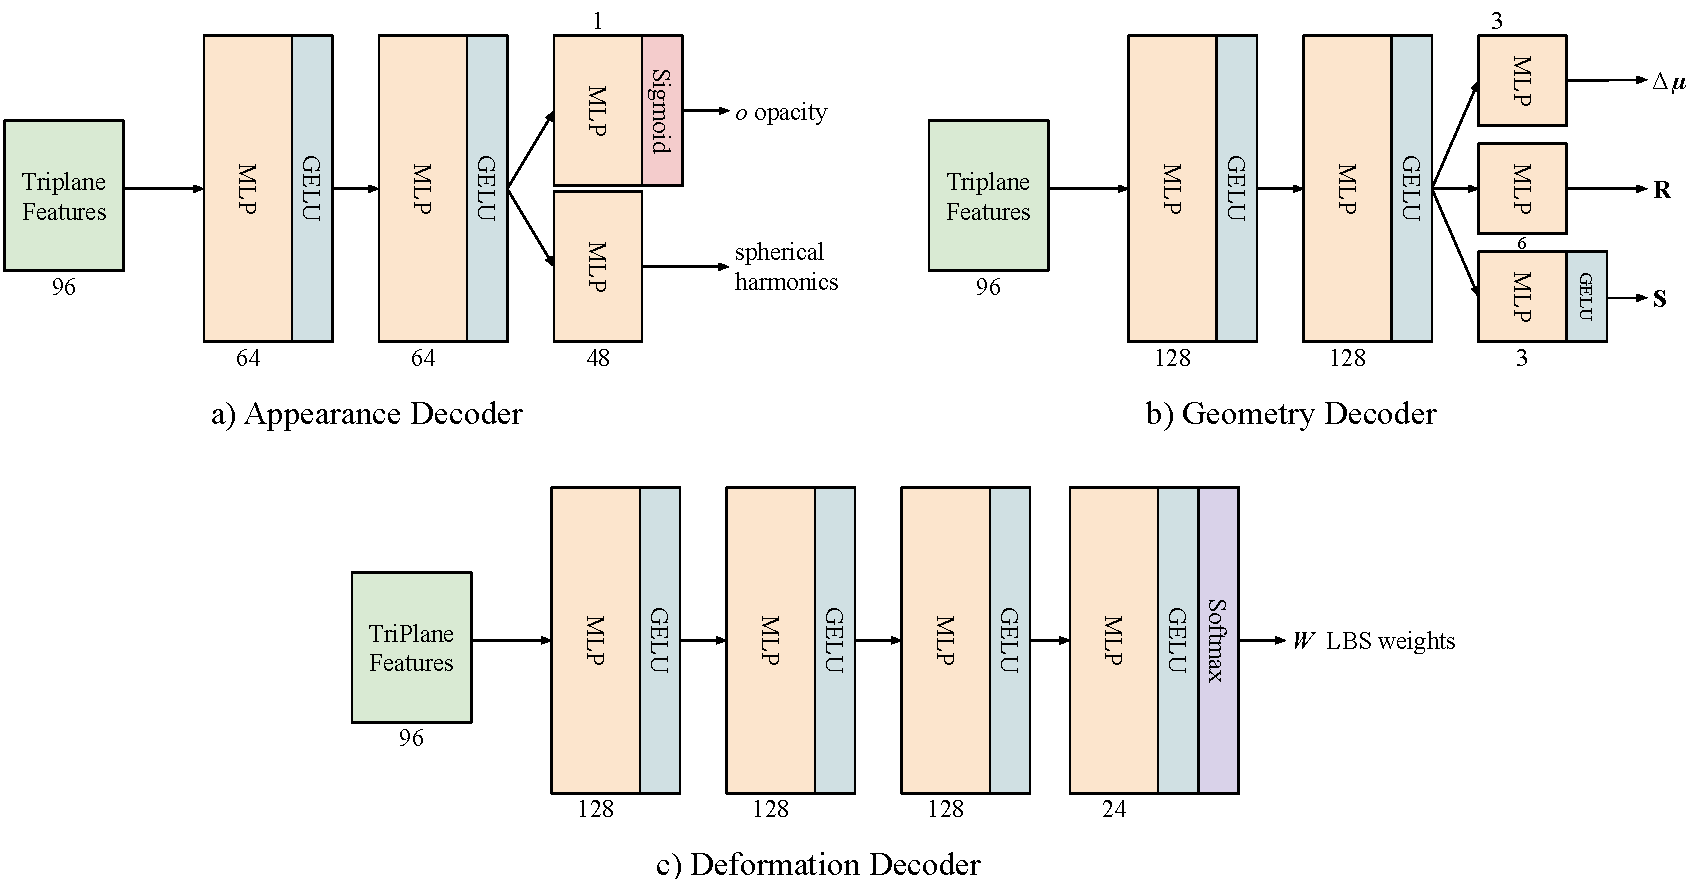
\includegraphics[width=\linewidth]{figures/pdf_files/network_architecture.pdf}
    \vspace{-7mm}
    \caption{\textbf{\acronym model architecture.} Here we show the network architecture of decoder models. 
    Appearance decoder $D_A$ is a 2-layer MLP with GELU~\cite{hendrycks2016gelu} activations. It takes triplane features as input and outputs opacity \& spherical harmonics parameters. Sigmoid activation function is used for opacity to constrain the values between $[0, 1]$. Geometry decoder $D_G$ also uses 2-layer MLP with GELU activation. It outputs the $\Delta \bm{\mu}, \bm{R}, \bm{S}$ for each Gaussians. We use GELU activation to ensure $\bm{S} \ge 0$. We do not need a normalization activation for $R$ unlike Kerbl \etal~\cite{kerbl3Dgaussians} since we use 6D rotation representation. We use a 3-layer MLP for deformation decoder $D_D$. It outputs the LBS weights. We apply a low-temperature softmax activation function with $T=0.1$ to ensure $\sum_{k=1}^{n_k} W_{k,i} = 1$. The use of a low temperature assists in predicting unimodal distributions, as most Gaussians need to be assigned to a single bone transformation.
    }
    \label{fig:netarch}
    \vspace{-2ex}
\end{figure*}{}
% We demonstrate a detailed view of the TriPlane-MLP model in \cref{fig:netarch} used to represent the human avatars. Our model use lightweight MLP models to decode the appearance, geometry, and deformation parameters of individual Gaussians. This helps us to train our model in a short amount of time without adding much overhead to the overall pipeline. We empirically found out that the GELU~\cite{hendrycks2016gelu} activation function lead to faster convergence. During rendering time Triplane and MLP models are discarded after predicting the canonical human avatar and its deformation parameters, which enables our method to perform fast rendering at 60 FPS.

We present a detailed overview of the triplane-MLP model in \cref{fig:netarch}, employed for representing human avatars. Our model utilizes lightweight MLP models to predict the appearance, geometry, and deformation parameters of individual Gaussians. This facilitates efficient model training within a short timeframe without significantly increasing the overall pipeline's computational burden. Through empirical investigation, we observed that the GELU activation function~\cite{hendrycks2016gelu} leads to quicker convergence. During the rendering phase, both triplane and MLP models are discarded once they predict the canonical human avatar and its deformation parameters. This design choice enables our method to achieve fast rendering at 60 FPS.

\paragraph{Appearance decoder ($D_A$)} comprises a 2-layer MLP with GELU activations~\cite{hendrycks2016gelu}. It takes triplane features as input and predicts opacity and spherical harmonics parameters. The opacity values are constrained within the range of $[0, 1]$ using a sigmoid activation function. Although no activation function is applied to the spherical harmonics parameters, the derived RGB values are clipped to be within $[0, 1]$ during the rasterization process.

\paragraph{Geometry decoder ($D_G$)} utilizes a 2-layer MLP with GELU activation, generating $\Delta \bm{\mu}, \bm{R}$, and $\bm{S}$ for each Gaussian. GELU activation ensures that $\bm{S} \ge 0$. Unlike Kerbl et al.~\cite{kerbl3Dgaussians}, we do not require a normalization activation for $\bm{R}$ as we employ a 6D rotation representation~\cite{Zhou_2019}.

\paragraph{Deformation decoder ($D_D$)} employs a 3-layer MLP to output LBS weights. We apply a low-temperature softmax activation function with $T=0.1$ to ensure $\sum_{k=0}^{n_k} \bm{W}_{k,i} = 1$. The use of a low temperature assists in predicting unimodal distributions, as most Gaussians need to be assigned to a single bone transformation.

\subsection{Loss implementation}
\paragraph{LBS regularization $\mathcal{L}_{\text{LBS}}$:} Given the limited set of training images, not regularizing LBS weights yields artifacts with unseen poses. Therefore, we apply regularization to ensure that the predicted LBS weights $\bm{W}$ closely align with those obtained from SMPL, employing an $\ell_2$ loss.

Specifically, to regularize the LBS weights $\bm{W}$, for individual Gaussians $\bm{p}_i$ we retrieve their $k=6$ nearest vertices on the \smpl mesh and take a distance-weighted average of their LBS weights to get $\hat{\bm{W}}$. The loss is $\mathcal{L}_{\text{LBS}} = \| \bm{W} - \hat{\bm{W}} \|_{\text{F}}^2$.

Following \cite{chen2021animatable,Zheng2020PaMIRPM} the distance-weighted average $\hat{\bm{W}_i}$ is obtained using:
\begin{align}
%\sum_{i \in \mathcal{N}(\bm{p}_i)}
    \hat{\bm{W}_i} &= \sum_{j \in \mathcal{N}_i}  \frac{\omega_j}{\omega} \bm{W}_j \label{eq:lbsquery}\\
    \omega_j &= \exp \left( {-\frac{\| \bm{p}_i - \bm{p}_j \| \| \bm{W}_i - \bm{W}_j \|}{2\sigma^2}} \right) \\
    \omega &= \sum_{j \in \mathcal{N}_i} \omega_j
\end{align}

where $\mathcal{N}_i$ is the $k$ nearest neighbor of $\bm{p}_i$. We use the efficient CUDA $k$-nn implementation of PyTorch3D library~\cite{ravi2020pytorch3d}.

% \subsection{SMPL pose parameters finetuning}
% We use off-the-shelf human pose and shape estimation models to obtain SMPL parameters. However, these models occasionally produce noisy estimates that do not align accurately with the observed human form. To address this misalignment between SMPL estimates and the actual human appearance, we incorporate joint optimization of SMPL pose parameters $\bm{\theta}$ and 3D Gaussians parameters during the training process. In Figure XXX, we illustrate the impact of online optimization on improving the accuracy of the estimates.

\subsection{Adaptive control of the number of 3D Gaussians}
We initialize the 3D Gaussians using a subdivided SMPL template with $n_v=110,210$ vertices. Despite the large number of vertices, the uniform subdivision across the body results in certain parts (e.g., face, hair, clothing) lacking sufficient points to represent high-frequency details. To address this issue, we adaptively control the number of 3D Gaussians during optimization, following a similar approach to Kerbl et al.~\cite{kerbl3Dgaussians}. The densification process starts after training the model for 3000 iterations, and subsequent densification steps are applied every 600 iterations.

% \section{Experiments}

\subsection{Ablation experiments}
\begin{figure*}[t]
    \centering
    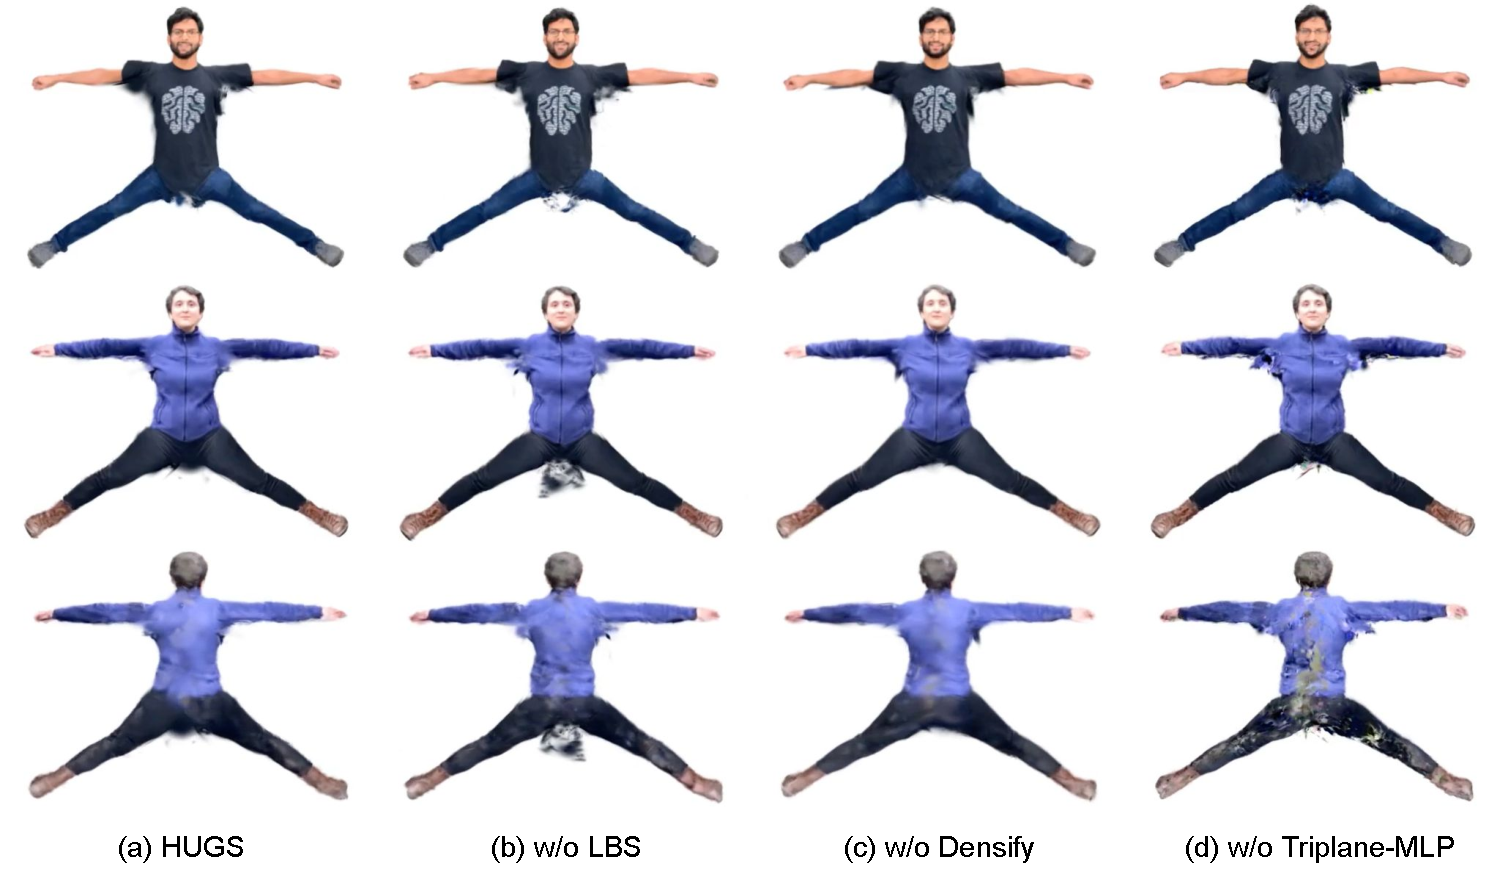
\includegraphics[width=\linewidth]{figures/pdf_files/ablation_supmat.pdf}
    \caption{\textbf{Ablation study} showing the visualization of details captured in the human canonical shape under different ablations of our method.} 
    \label{fig:ablation_supmat}
\end{figure*}

In this section, we provide a detailed explanation of the ablation experiments.

\paragraph{w/o LBS baseline.} We replace the learned LBS weights with the SMPL LBS weights to assess the significance of learnable deformation. We obtain the SMPL LBS weights for a query point $\bm{p}_i$ using \cref{eq:lbsquery}. As the $k$-nn (k-nearest neighbors) approach can be ambiguous for points around the intersection of joints, utilizing SMPL weights may result in artifacts, particularly visible in areas around these intersections, as illustrated in (a) and (b) columns in \cref{fig:ablation_supmat}.

\paragraph{w/o Densify.} In this ablation experiment, we maintain a fixed number of Gaussians throughout the optimization process. The results of this experiment are depicted in the (a) and (c) columns in \cref{fig:ablation_supmat}. The \textit{w/o Densify} setting leads to certain Gaussians protruding from the body, resulting in a suboptimal reconstruction of details, as evidenced by the example of boot laces in the second row.

\paragraph{w/o triplane-MLP baseline.} In this ablation experiment, we directly optimize the 3D Gaussian parameters instead of learning them with a trilane-MLP model. To deform individual Gaussians, we utilize the SMPL LBS weights obtained using the query algorithm presented in \cref{eq:lbsquery}. The results of this experiment are displayed in the (a) and (d) columns in \cref{fig:ablation_supmat}. As each Gaussian is optimized independently, the per-Gaussian colors have a tendency to overfit to the training frames, leading to color artifacts. This results in poor quality on novel animation renderings and test frames. On the other hand, triplane-MLP provides implicit regularization to the color as a function of Gaussian position. Also, the learned appearance provides additional 3D supervision signal for the positions of the Gaussians.

\paragraph{w/o Joint human \& scene optimization.} We assess the impact of jointly optimizing the human and scene models in this ablation experiment. Our final model, HUGS, represents human and scene Gaussians separately, however the optimization is performed jointly. An alternative approach involves initially optimizing the scene by masking out human regions and then optimizing the human Gaussians. This strategy aligns with the approach used in NeuMan~\cite{jiang2022neuman}. However, as illustrated in column (b) of \cref{fig:ablation_joint_opt}, this alternative strategy results in floating Gaussians in the scene due to sparse input views. On the contrary, when human and scene optimization is performed jointly, the human serves as a constraint for the scene reconstruction, mitigating the occurrence of floaters and yields cleaner rendered images as displayed in column (a) of \cref{fig:ablation_joint_opt}.

% We ablate the impact of jointly optimizing the human and scene models. Our final model HUGS represented human and scene Gaussians separately; however optimization is performed jointly. An alternative to this is to first optimize the scene by masking out human regions and then optimize the human Gaussians. This is the strategy employed in NeuMan~\cite{jiang2022neuman}. However as shown in \cref{fig:ablation_joint_opt} this strategy leads to floating Gaussians in the scene. This is because of sparse input views. However when jointly optimizing human and scene yields, human constrains the scene reconstruction to mitigate the floaters.
% Left is the result of optimizing the human and scene model jointly. Right is the result of optimizing the scene first and then optimizing the human model. Overall human movement helps to constrain the scene geometry. This leads to a more accurate human and scene reconstruction.

\begin{figure*}[t]
    \centering
    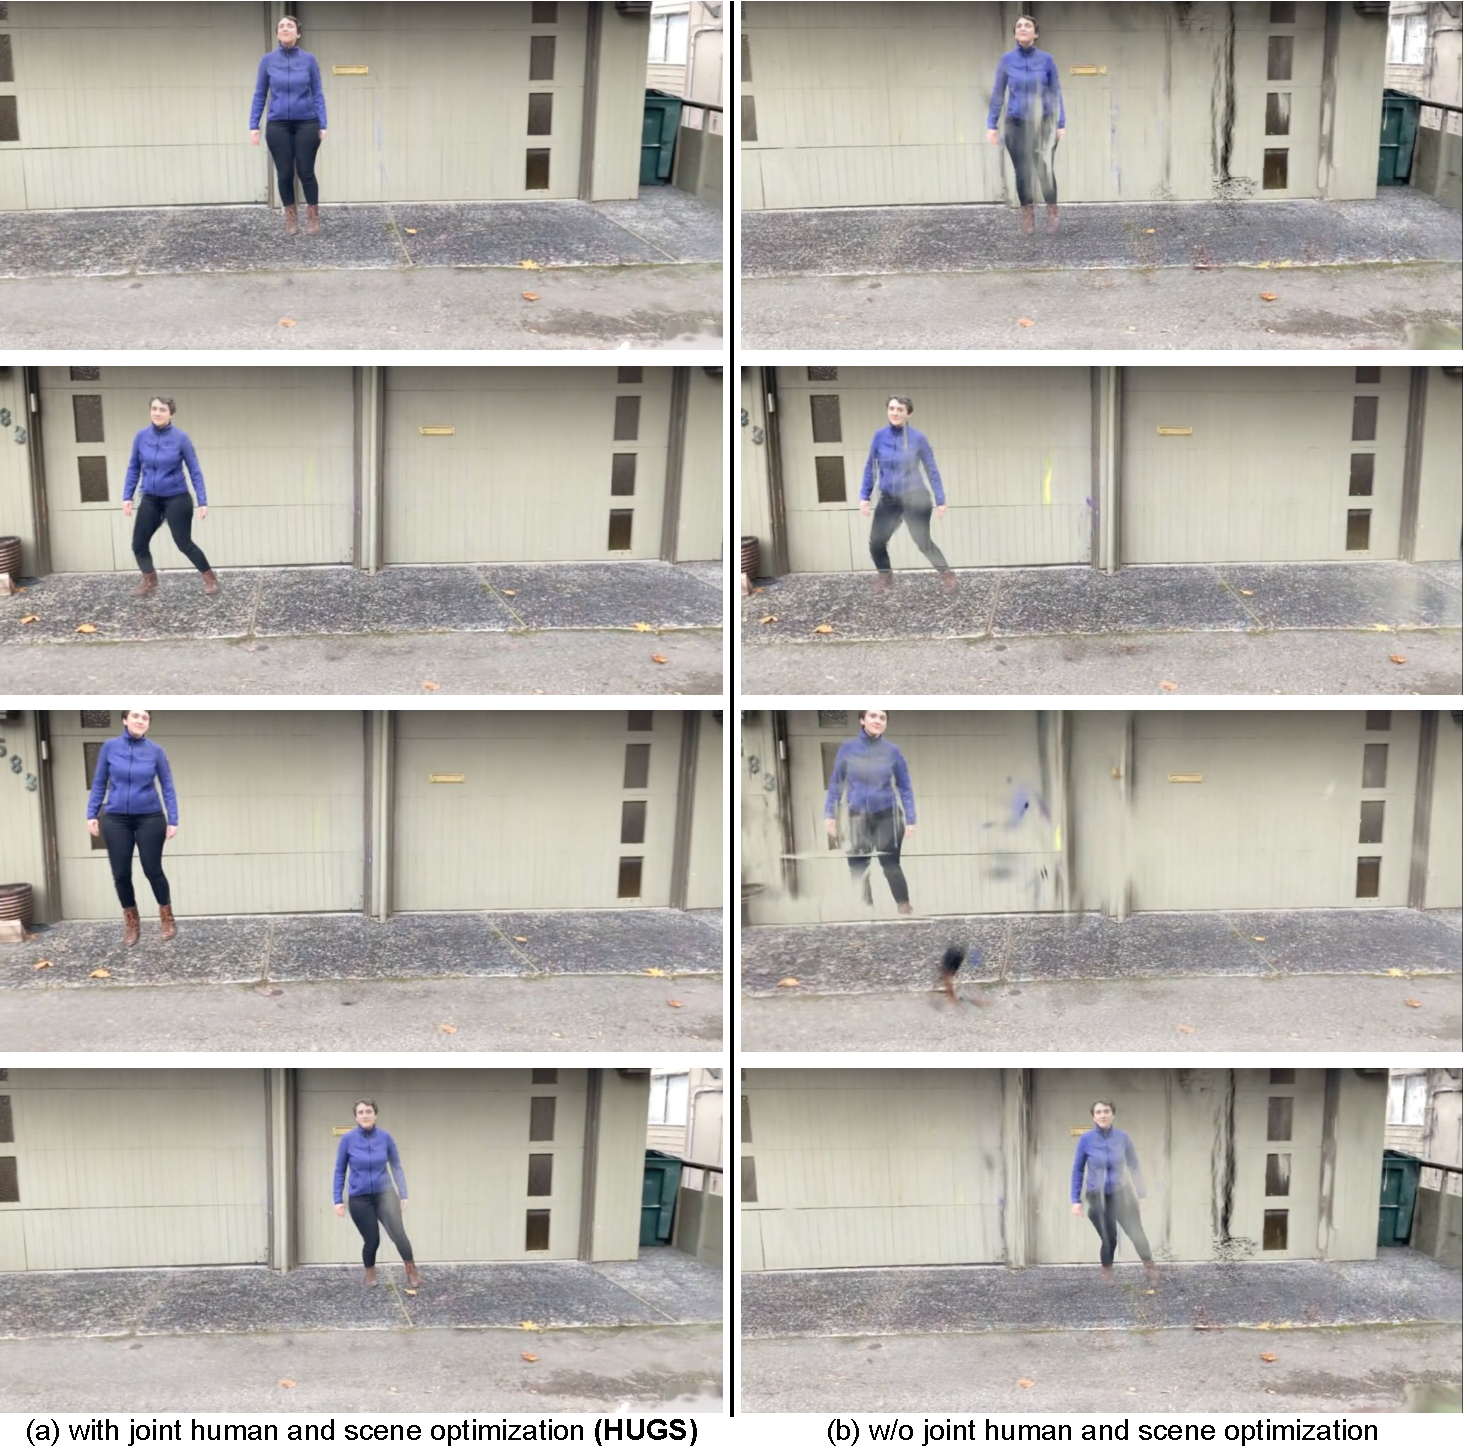
\includegraphics[width=\linewidth]{figures/pdf_files/ablation_joint_opt.pdf}
    \caption{\textbf{Ablation study} showing the impact of jointly optimizing the human and scene models. Left column (a) shows the result of our method HUGS with joint optimization of human and scene Gaussians. Right column (b) shows optimizing the scene first by masking out the human regions and then optimizing the human Gaussians.} 
    \label{fig:ablation_joint_opt}
\end{figure*}

\subsection{Novel animation renderings}

In \cref{fig:posed_renders}, we present novel animation renderings featuring subjects from the NeuMan dataset~\cite{jiang2022neuman}. Additionally, \cref{fig:novel_scene_pose} showcases the composition of multiple animated subjects in various scenes, with poses obtained from the AMASS motion capture dataset~\cite{AMASS:ICCV:2019}. For a more extensive collection of video results demonstrating novel pose and scene animations, please refer to our supplementary webpage.

\begin{figure*}[t]
    \centering
    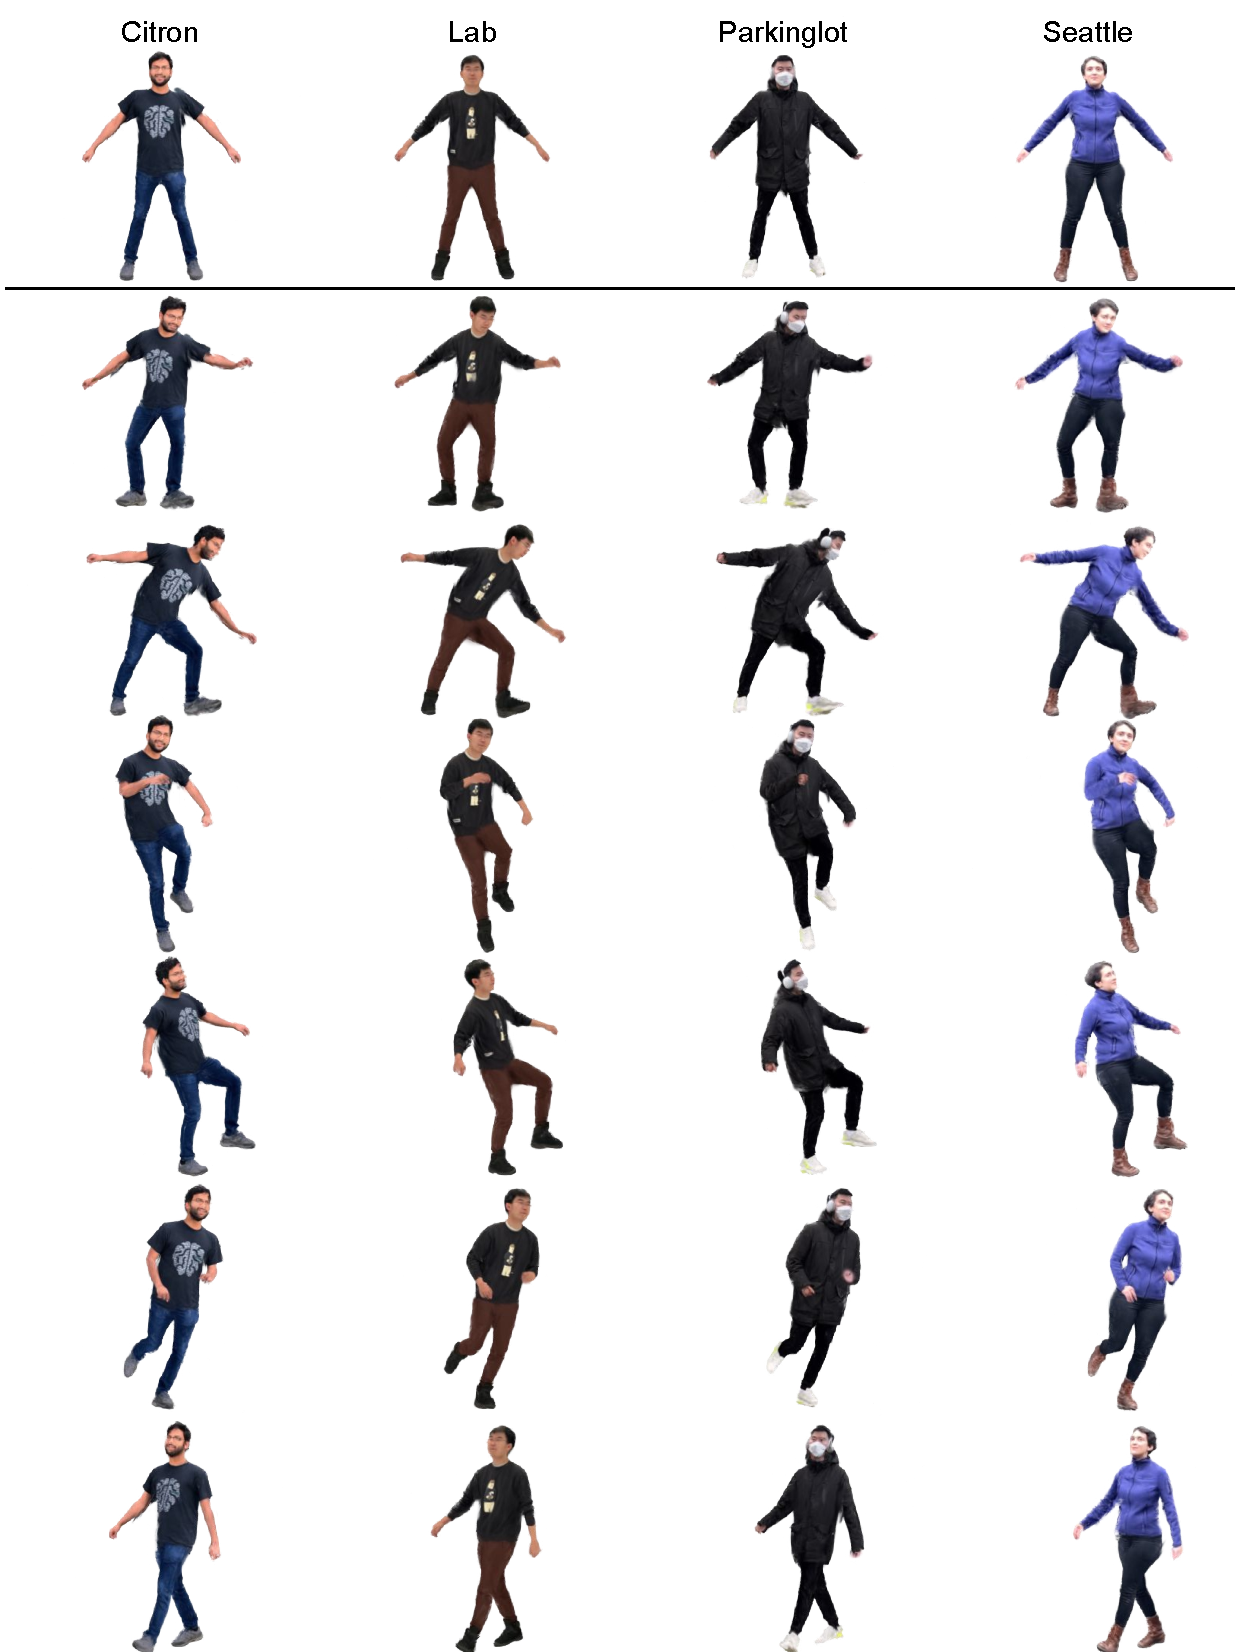
\includegraphics[width=0.9\linewidth]{figures/pdf_files/posed_imgs.pdf}
    \caption{\textbf{Novel pose renderings} We demonstrate the novel pose renderings of subjects (top row) from the NeuMan dataset.} 
    \label{fig:posed_renders}
\end{figure*}{}
\begin{figure*}[t]
    \centering
    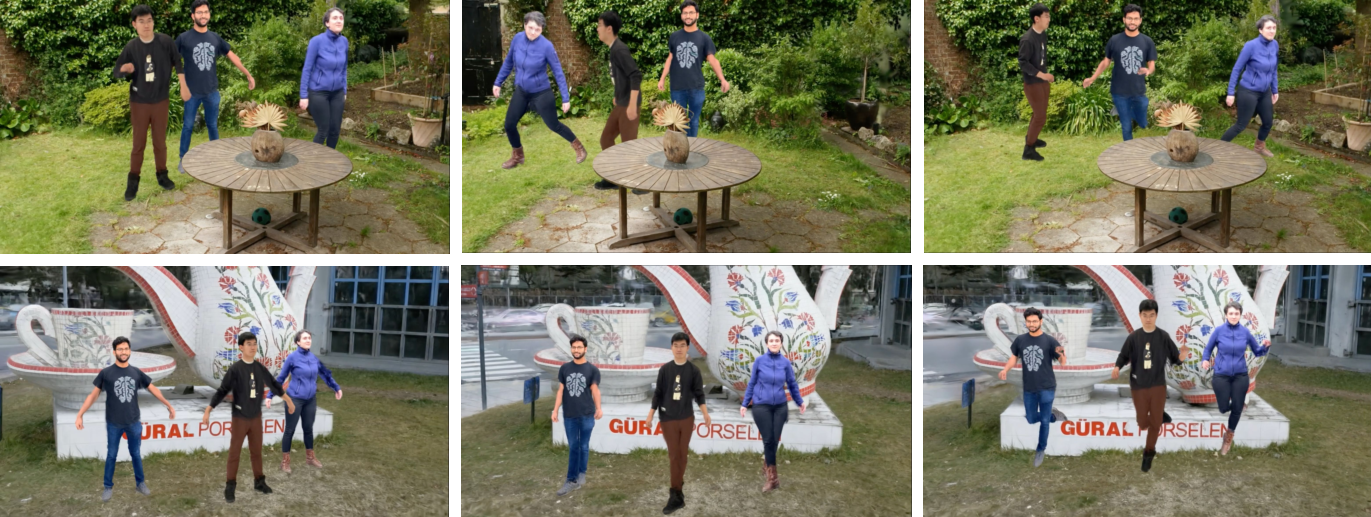
\includegraphics[width=\linewidth]{figures/pdf_files/novel_scene_pose.pdf}
    \caption{\textbf{Animation of multiple people in novel scenes.} Renderings obtained by transferring the Human Gaussians to different scenes.}
    \label{fig:novel_scene_pose}
\end{figure*}{}



\end{document}
